\documentclass[10pt]{article}
\usepackage[margin=1in]{geometry}
% This is the preamble, load any packages you're going to use here
% \usepackage{physics} % provides lots of nice features and commands often used in physics, it also loads some other packages (like AMSmath)
\usepackage{siunitx} % typesets numbers with units very nicely
\usepackage{enumerate} % allows us to customize our lists
\usepackage{hyperref}
\usepackage{xcolor}
\usepackage{graphicx}
\usepackage[version=4]{mhchem}
\usepackage{siunitx}
\usepackage{enumitem}
\usepackage{float} % Include this in the preamble
\usepackage[most]{tcolorbox}
\setlength{\parskip}{0.75em}
\tcbuselibrary{skins}
\newtcolorbox{explorationbox}[1][]{%
  enhanced,
  colback=blue!10,
  colframe=blue!50!black,
  fonttitle=\bfseries,
  left=20pt,
  title=Questions for further exploration:,
  #1
}
\newtcolorbox{warningbox}[1][]{%
  enhanced,
  colback=red!10,          % Light reddish background
  colframe=red!50!black,   % Darker red frame
  fonttitle=\bfseries,
  title=Warning:,          % Title of the box
  #1
}
\usepackage{fancyhdr} % Include the package
\renewcommand{\labelitemi}{--}
\pagestyle{fancy} % Enable fancy page style
\fancyhf{} % Clear existing header and footer
\rhead{Anton Morgunov} % Add your name to the right side of the header
\lhead{CHEM 573 Final Report} % Left side of the header
\cfoot{\thepage/10} % Center of the footer (page number)


\begin{document}

% \title{\textbf{Exploring the Algorithmic Instructions Sufficient for Thermalization in Gas Phase}}
% \author{Anton Morgunov}
% \date{\today}

\noindent\hrule height 2pt % Thicker horizontal line
\vspace{0.5em} % Space after the thick line

\begin{center}
    {\Large \textbf{Exploring the Algorithmic Instructions Sufficient for Equilibration}} \\
    \vspace{1em} % Space between title and author name
    {\large Anton Morgunov}. {\large \today}
    % \vspace{0.5em} % Space between author name and email
    % {\small \texttt{anton.morgunov@email.com}}\\ % Your email
    % \vspace{1em} % Space between email and date
\end{center}

\vspace{0.5em} % Space before the thin line
\noindent\hrule height 1pt % Thinner horizontal line

% \maketitle

% \begin{abstract}

% \end{abstract}

\section{Motivation}
In statistical mechanics, we try to derive macroscopic variables through properties of individual components such as atoms or molecules. Those macroscopic variables, however, are end results (after all, there is no concept of time in thermodynamics). This project aimed to explore the mechanism by which that end result is achieved. Particularly, we wanted to explore the minimal set of instructions that would result in the equilibration (both entropical and thermal) of a system with two kinds of particles (potentially with different masses and temperatures), initially placed in different compartments of a box. A big focus of this project was to create a software for the visualization of not just simulation results, but of the simulation itself. Although such visualizations are often overlooked in favor of analyzing numerical results, we believe having a visual representation of how molecules actually behave is profound for training the intuition, which is what, quite often implicitly, guides scientists in their research.

This report is structured as follows:\vspace{-1em}
\begin{itemize}
    \itemsep-0.2em
    \item In Section \ref{sec:methods-brief}, we provide a brief overview of methodology necessary to appreciate the results.
    \item In Section \ref{sec:results}, we present and discuss those results.
    \item In Section \ref{sec:public-api}, we describe the public API of the code so that the reader can play and explore the simulation.
    \item In Section \ref{sec:changelog} we highlight the work that was done since the intermediate report back in CHEM 572.
    \item Finally, in section \ref{sec:methods-detailed}, we provide a more detailed description of the code and the methods used.
\end{itemize}

The code for this simulation is published on \href{https://github.com/anmorgunov/statmech-simulation}{\textcolor{blue}{Github}}. 

\section{Methods Overview}
\label{sec:methods-brief}
Because of inherent focus on developing chemical intuition, we believe it is worth mentioning that in the process of working on this project, the author discovered his confusion of the map and the territory. Particularly, we mistakenly believed the \textit{Brownian Motion} is the actual mechanism by which particles move in a container. Fairly quickly we realized that it would be impossible to satisfy conservation of momentum and energy if particles changed their velocity abruptly. Therefore, we decided to give all particles same magnitude of initial velocity with randomly initialized directions, and let each particle move on a steady course until it collides with another particle. Collisions are resolved by treating them as perfectly elastic. 

The kinetic energy of all particles at any given timestep is used to calculate the temperature of the system (by making an assumption that the total kinetic energy is determined by the equipartition theorem). The fraction of atoms initially placed exclusively in a right container is monitored throughout the simulation. The magnitudes of all particles are monitored throughout the simulation. In addition, we keep track of the angle (determined as $\theta = \arctan v_x/v_y$) of velocity of a single particle.

Next we wanted to assess whether we could have modeled the given number of particles at a given temperature by implementing the Brownian motion, i.e. doing the random walk. Because in a random walk implementation the angles of velocities are drawn from a uniform distribution at each timestemp, one way of assessing whether the random walk is a valid model for the mechanism of movement is to check whether the distribution of angles when the movement is determined by physical collisions is uniform. Because we initialize all particles by setting a fixed magnitude of velocity and a random angle, the distribution of angles over all particles would be uniform regardless of the number of particles and temperature. Therefore, we decided to keep track of angles at each timestep of a single, randomly chosen particle. We then bin those angles into 10 equally distributed bins and assess whether the distribution is close enough to uniform. We do this by computing the p-value of the Kolmogorov-Smirnov test, the p-value of the chi-squared test, and the p-value of the relaxed chi-squared test (which does not penalize deviations from uniformity of 5\% and less).

Finally, we wanted to determine if thermalization could occur even if we introduce a physical barrier between particles. Evidently, a plain impermeable barrier would simply reflect all particles. Therefore, we decided to model a physical barrier by creating an object, which can absorb, store, and emit energy when particles collide with it. Specifically, the average kinetic energy of a cooler set of particles determines the maximum capacity of the \texttt{EnergyWall} and the object keeps track of the moving average ($\alpha=0.5$) of kinetic energy of particles which collide with it. If the wall is not full and a particle with larger kinetic energy than the moving average collides with it, a 10\% of the kinetic energy is absorbed by the wall. If the wall is full and the particle's kinetic energy is smaller than the moving average, the wall emits 10\% of the kinetic energy. In all other cases, the particles bounce off the wall without any change in their kinetic energy.

\section{Results \& Discussion}
\label{sec:results}
The first major observed result is that even if all particles being with the same magnitude of velocity, fairly quickly the distribution of velocities becomes Maxwell-Boltzmann (Figure \ref{fig:speed_thermalization}). In essence, this means that the mechanism for thermalization is the collisions between particles. 

\begin{figure}[h]
    \centering
    \begin{minipage}{0.4\linewidth}
        \includegraphics[width=\linewidth]{../figures/jpg/speed/init2.jpg}
    \end{minipage}
    \begin{minipage}{0.4\linewidth}
        \includegraphics[width=\linewidth]{../figures/jpg/speed/tr2-t93.jpg}
    \end{minipage} \\
    \begin{minipage}{0.4\linewidth}
        \includegraphics[width=\linewidth]{../figures/jpg/speed/tr2-t527.jpg}
    \end{minipage}
    \begin{minipage}{0.4\linewidth}
        \includegraphics[width=\linewidth]{../figures/jpg/speed/tr2-t2863.jpg}
    \end{minipage}
    \caption{Thermalization of carbon and oxygen atoms initially prepared at $T=\qty{100}{K}$ and $T=\qty{500}{K}$, respectively. The top right, bottom left, and bottom right panels show the state of the system at timesteps $t=93$, $t=527$, and $t=2863$, respectively.}
    \label{fig:speed_thermalization}
\end{figure}

The second major result is that, as expected, the particles diffuse until they are distributed uniformly in the whole container, meaning that the fraction of particles in both compartments is equal to $0.5$ (Figure \ref{fig:compartment_fractions}). As that happens, the temperature of the system fluctuates by around 10\% around the average temperature (Figure \ref{fig:temperature_evolution}).

The third major result is that the distribution of angles of velocities of a single particle becomes closer to the uniform distribution as temperature increases (Figure \ref{fig:uniformity_confidence}). Notably, both chi-squared and Kolmogorov-Smirnov tests are very sensitive to even small deviations from uniformity, and so the p-values determined by those metrics do not agree with a qualitative assessment of the actual distribution of angles. In contrast, the relaxed chi-squared test outputs a p-value which agrees more with the qualitative assessment of the distribution of angles, thereby justifying our choice of this metric for further analysis. If we run the simulation for 5000 steps for different number of particles and different initial temperatures, and then calculate the average p-value over the last 100 timesteps, we see that, as expected, the random walk becomes a valid model with large number of particles and large temperatures. Notably, once you get to 10 000 particles, even at room temperature the random walk becomes a valid model (Figure \ref{fig:uniformity_summary}).

Finally, we find that as long as the barrier between compartments is capable of absorbing and emitting energy, the two sets of particles thermalize (Figure \ref{fig:rigid_wall}) even without direct contact.

\section{Public API}
\label{sec:public-api}
To run simulations, all you need is to type \texttt{python server.py} into the terminal. This will start a server on \texttt{localhost:5000}. You can then open \texttt{localhost:5000} in your browser and start the simulation. Optionally, you can pass the following parameters along with the command in the terminal:
\begin{itemize}
    \itemsep-0.5em
    \item \texttt{-h} - print the help message, highlighting the available parameters
    \item \texttt{-nl} or \texttt{--numleft} - number of particles initially placed in the left compartment
    \item \texttt{-nr} or \texttt{--numright} - number of particles initially placed in the right compartment
    \item \texttt{-la} or \texttt{--leftatom} - element which is initially placed in the left compartment
    \item \texttt{-ra} or \texttt{--rightatom} - element which is initially placed in the right compartment
    \item \texttt{-lt} or \texttt{--lefttemp} - initial temperature of particles in the left compartment
    \item \texttt{-rt} or \texttt{--righttemp} - initial temperature of particles in the right compartment
    \item \texttt{-u} or \texttt{--updatefrequency} - how often should the statistics of the simulation be updated (in timesteps)
    \item \texttt{-qt} or \texttt{--quadtree} - whether to use quadtree data structure for more efficient collision detection
    \item \texttt{-rw} or \texttt{--rigidwall} - whether to use rigid wall that only permits energy exchange
\end{itemize}
These parameters could be provided in any order. \texttt{-rw} and \texttt{-qt} parameters are passed on their own without extra arguments, while all other parameters require an argument. For example, to run the simulation with 1000 carbon atoms at $T=\qty{300}{K}$ initially placed in the left compartment and 1000 oxygen atoms at $T=\qty{400}{K}$ initially placed in the right compartment, with statistics updated every 100 timesteps, and with rigid wall that only permits energy exchange, you would type \texttt{python server.py -nl 1000 -nr 1000 -la C -ra O -lt 300 -rt 4000 -u 100 -rw}. An extra \texttt{-qt} parameter significantly improves the performance of the simulation when more than 150 atoms cumulatively are used.

\newpage

\begin{figure}[H]
    \centering
    \begin{minipage}{0.43\linewidth}
        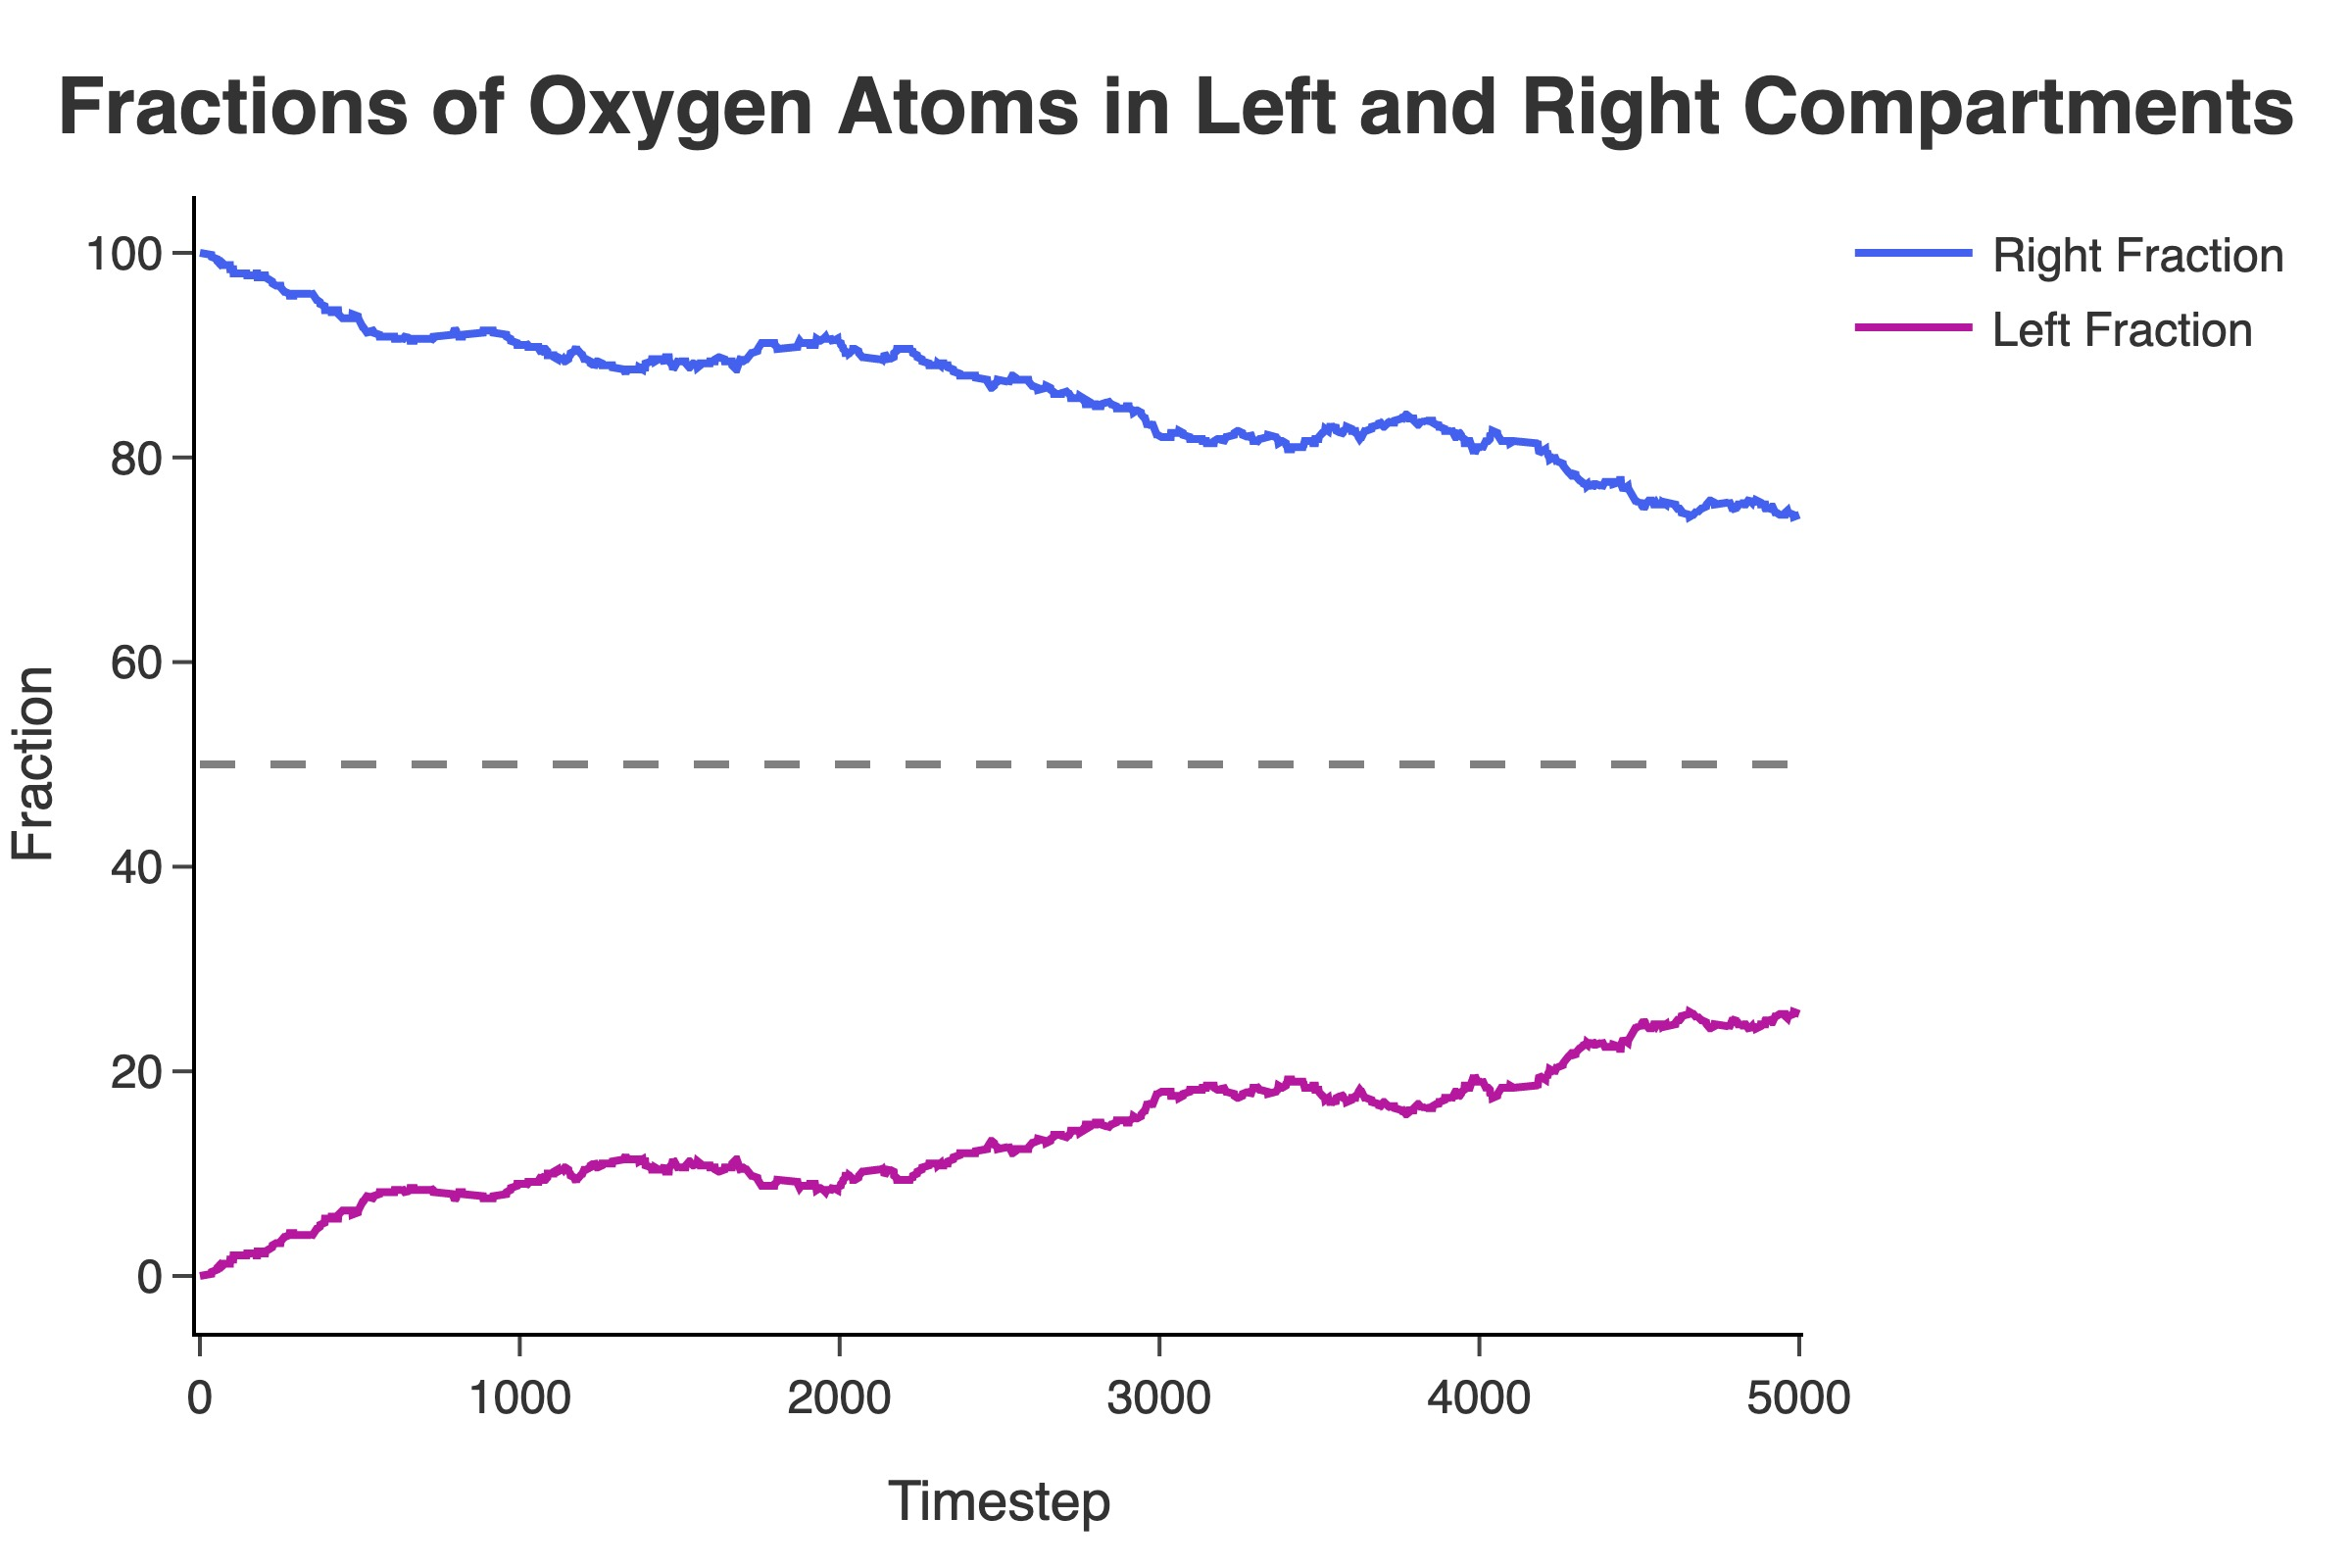
\includegraphics[width=\linewidth]{../figures/jpg/distribution/atoms_1000_temp_300_compartment_fractions.jpg}
    \end{minipage}
    \begin{minipage}{0.43\linewidth}
        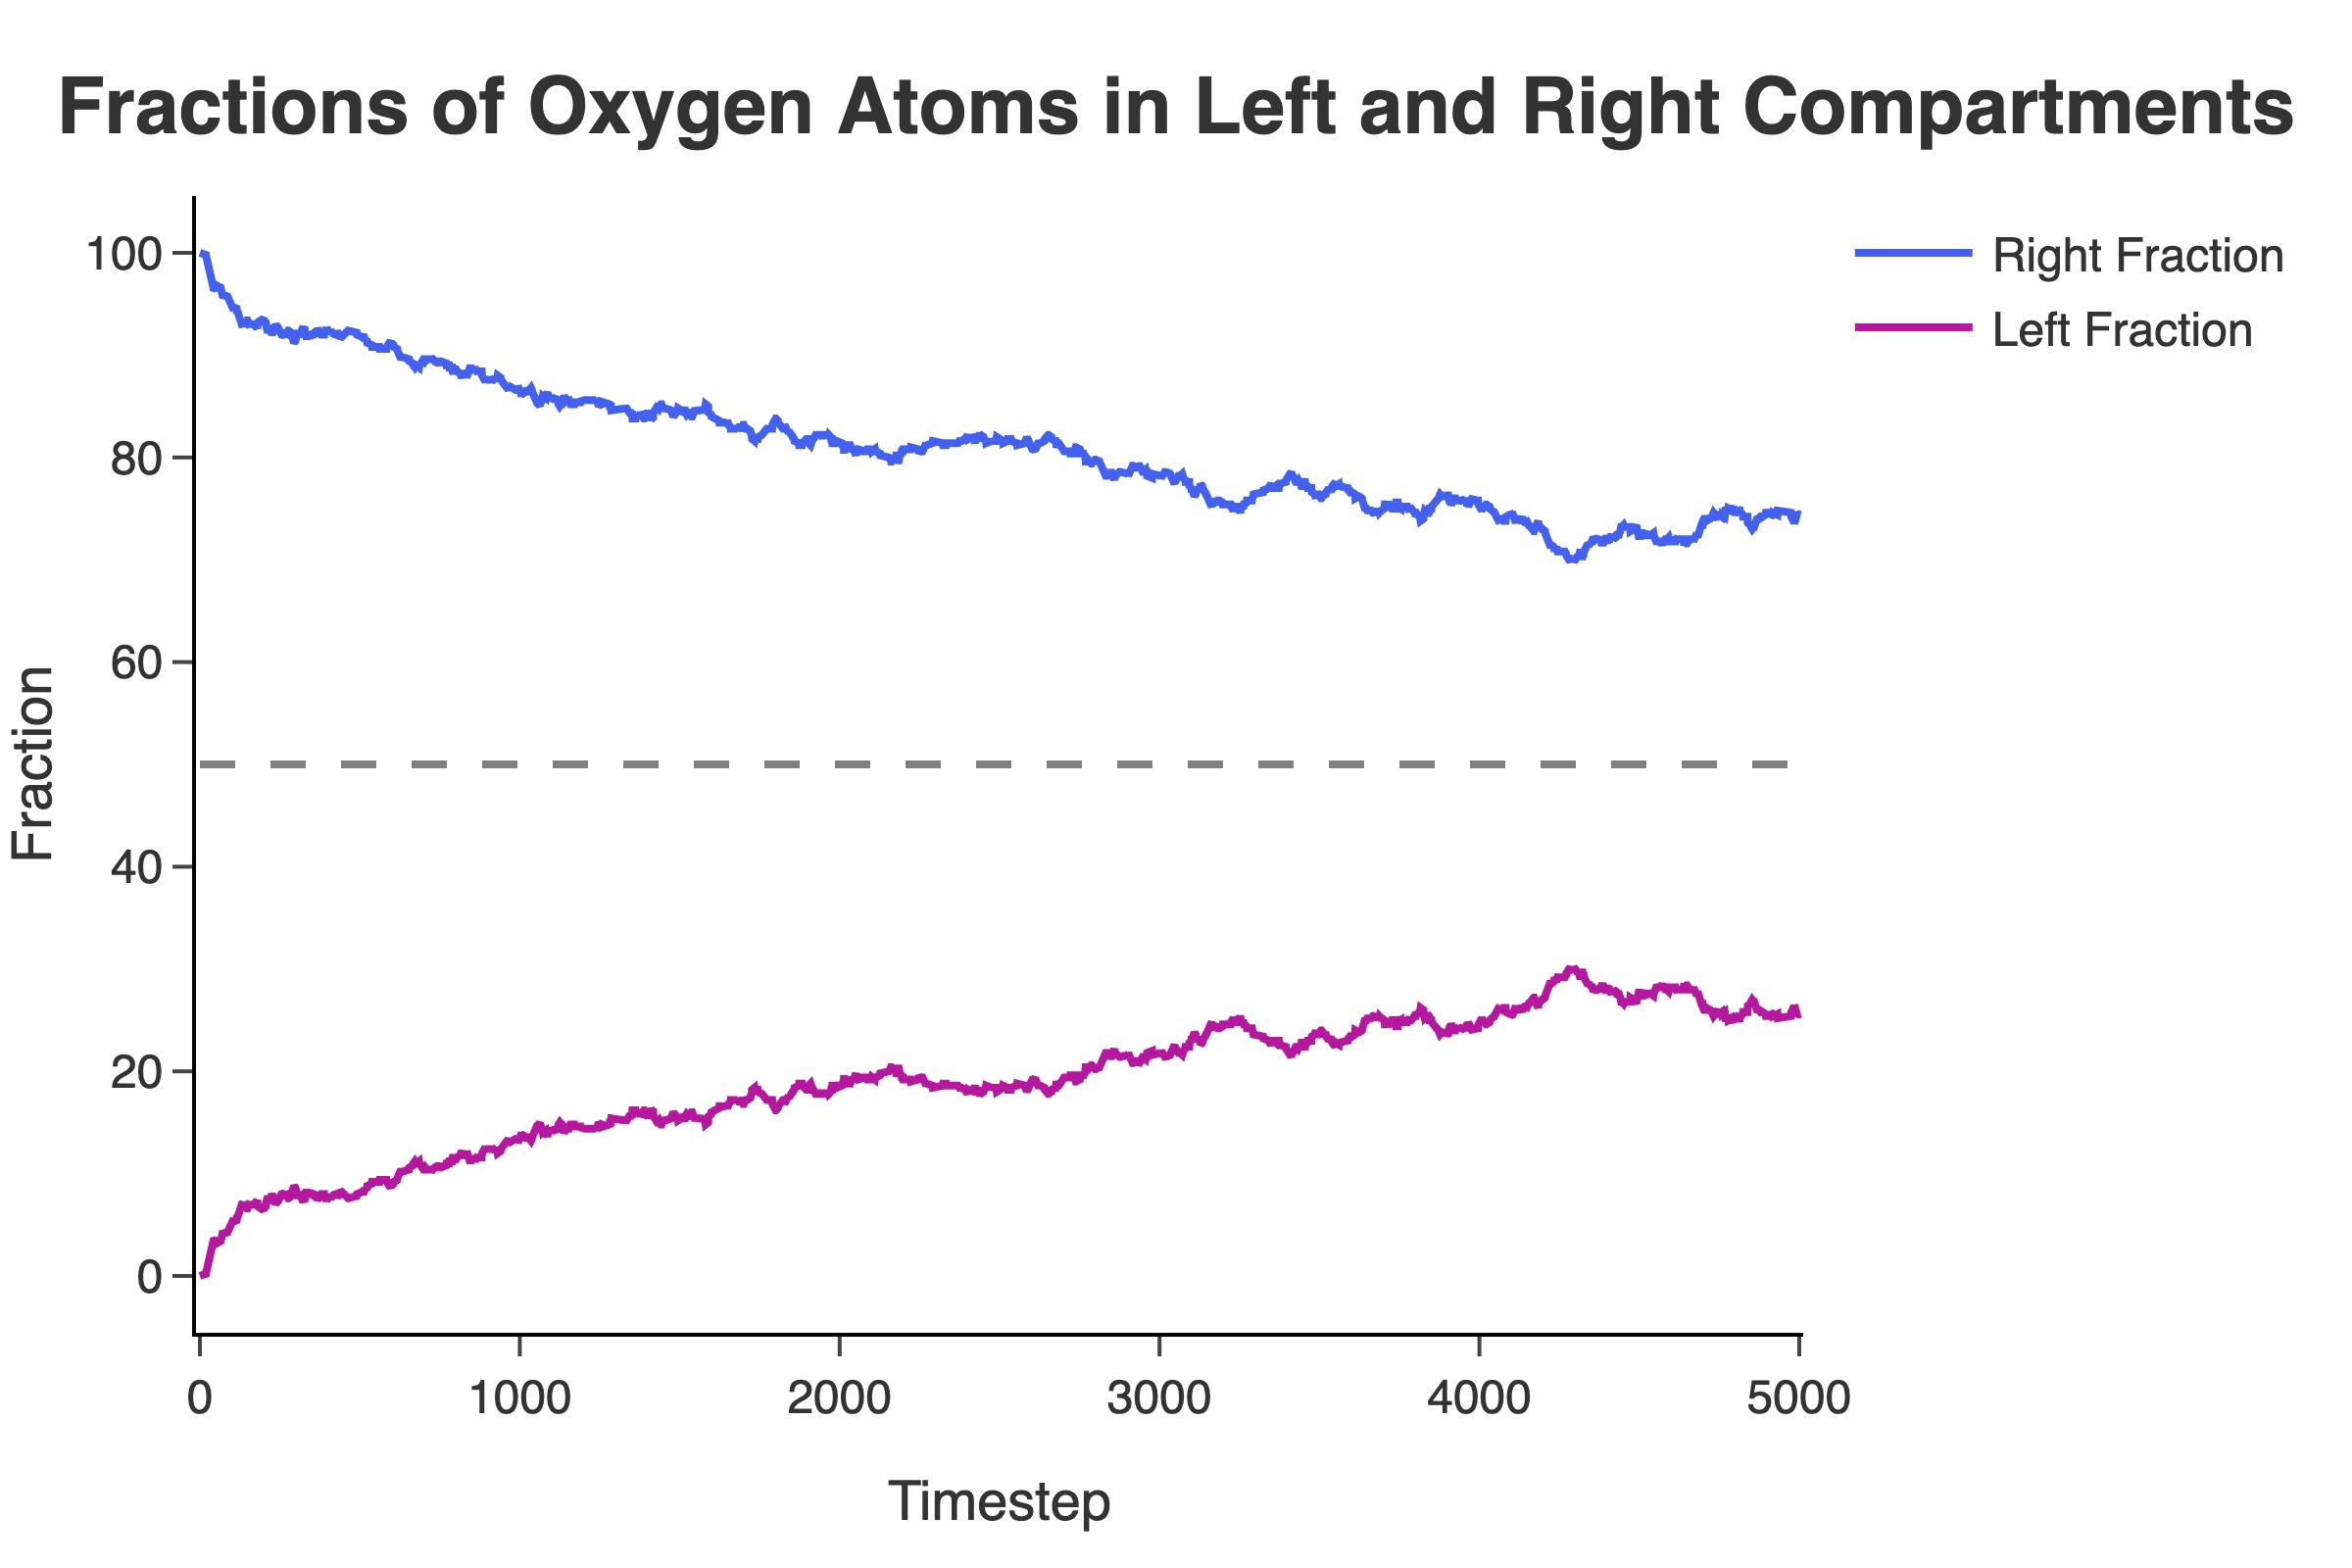
\includegraphics[width=\linewidth]{../figures/jpg/distribution/atoms_1000_temp_1000_compartment_fractions.jpg}
    \end{minipage} \\
    \begin{minipage}{0.43\linewidth}
        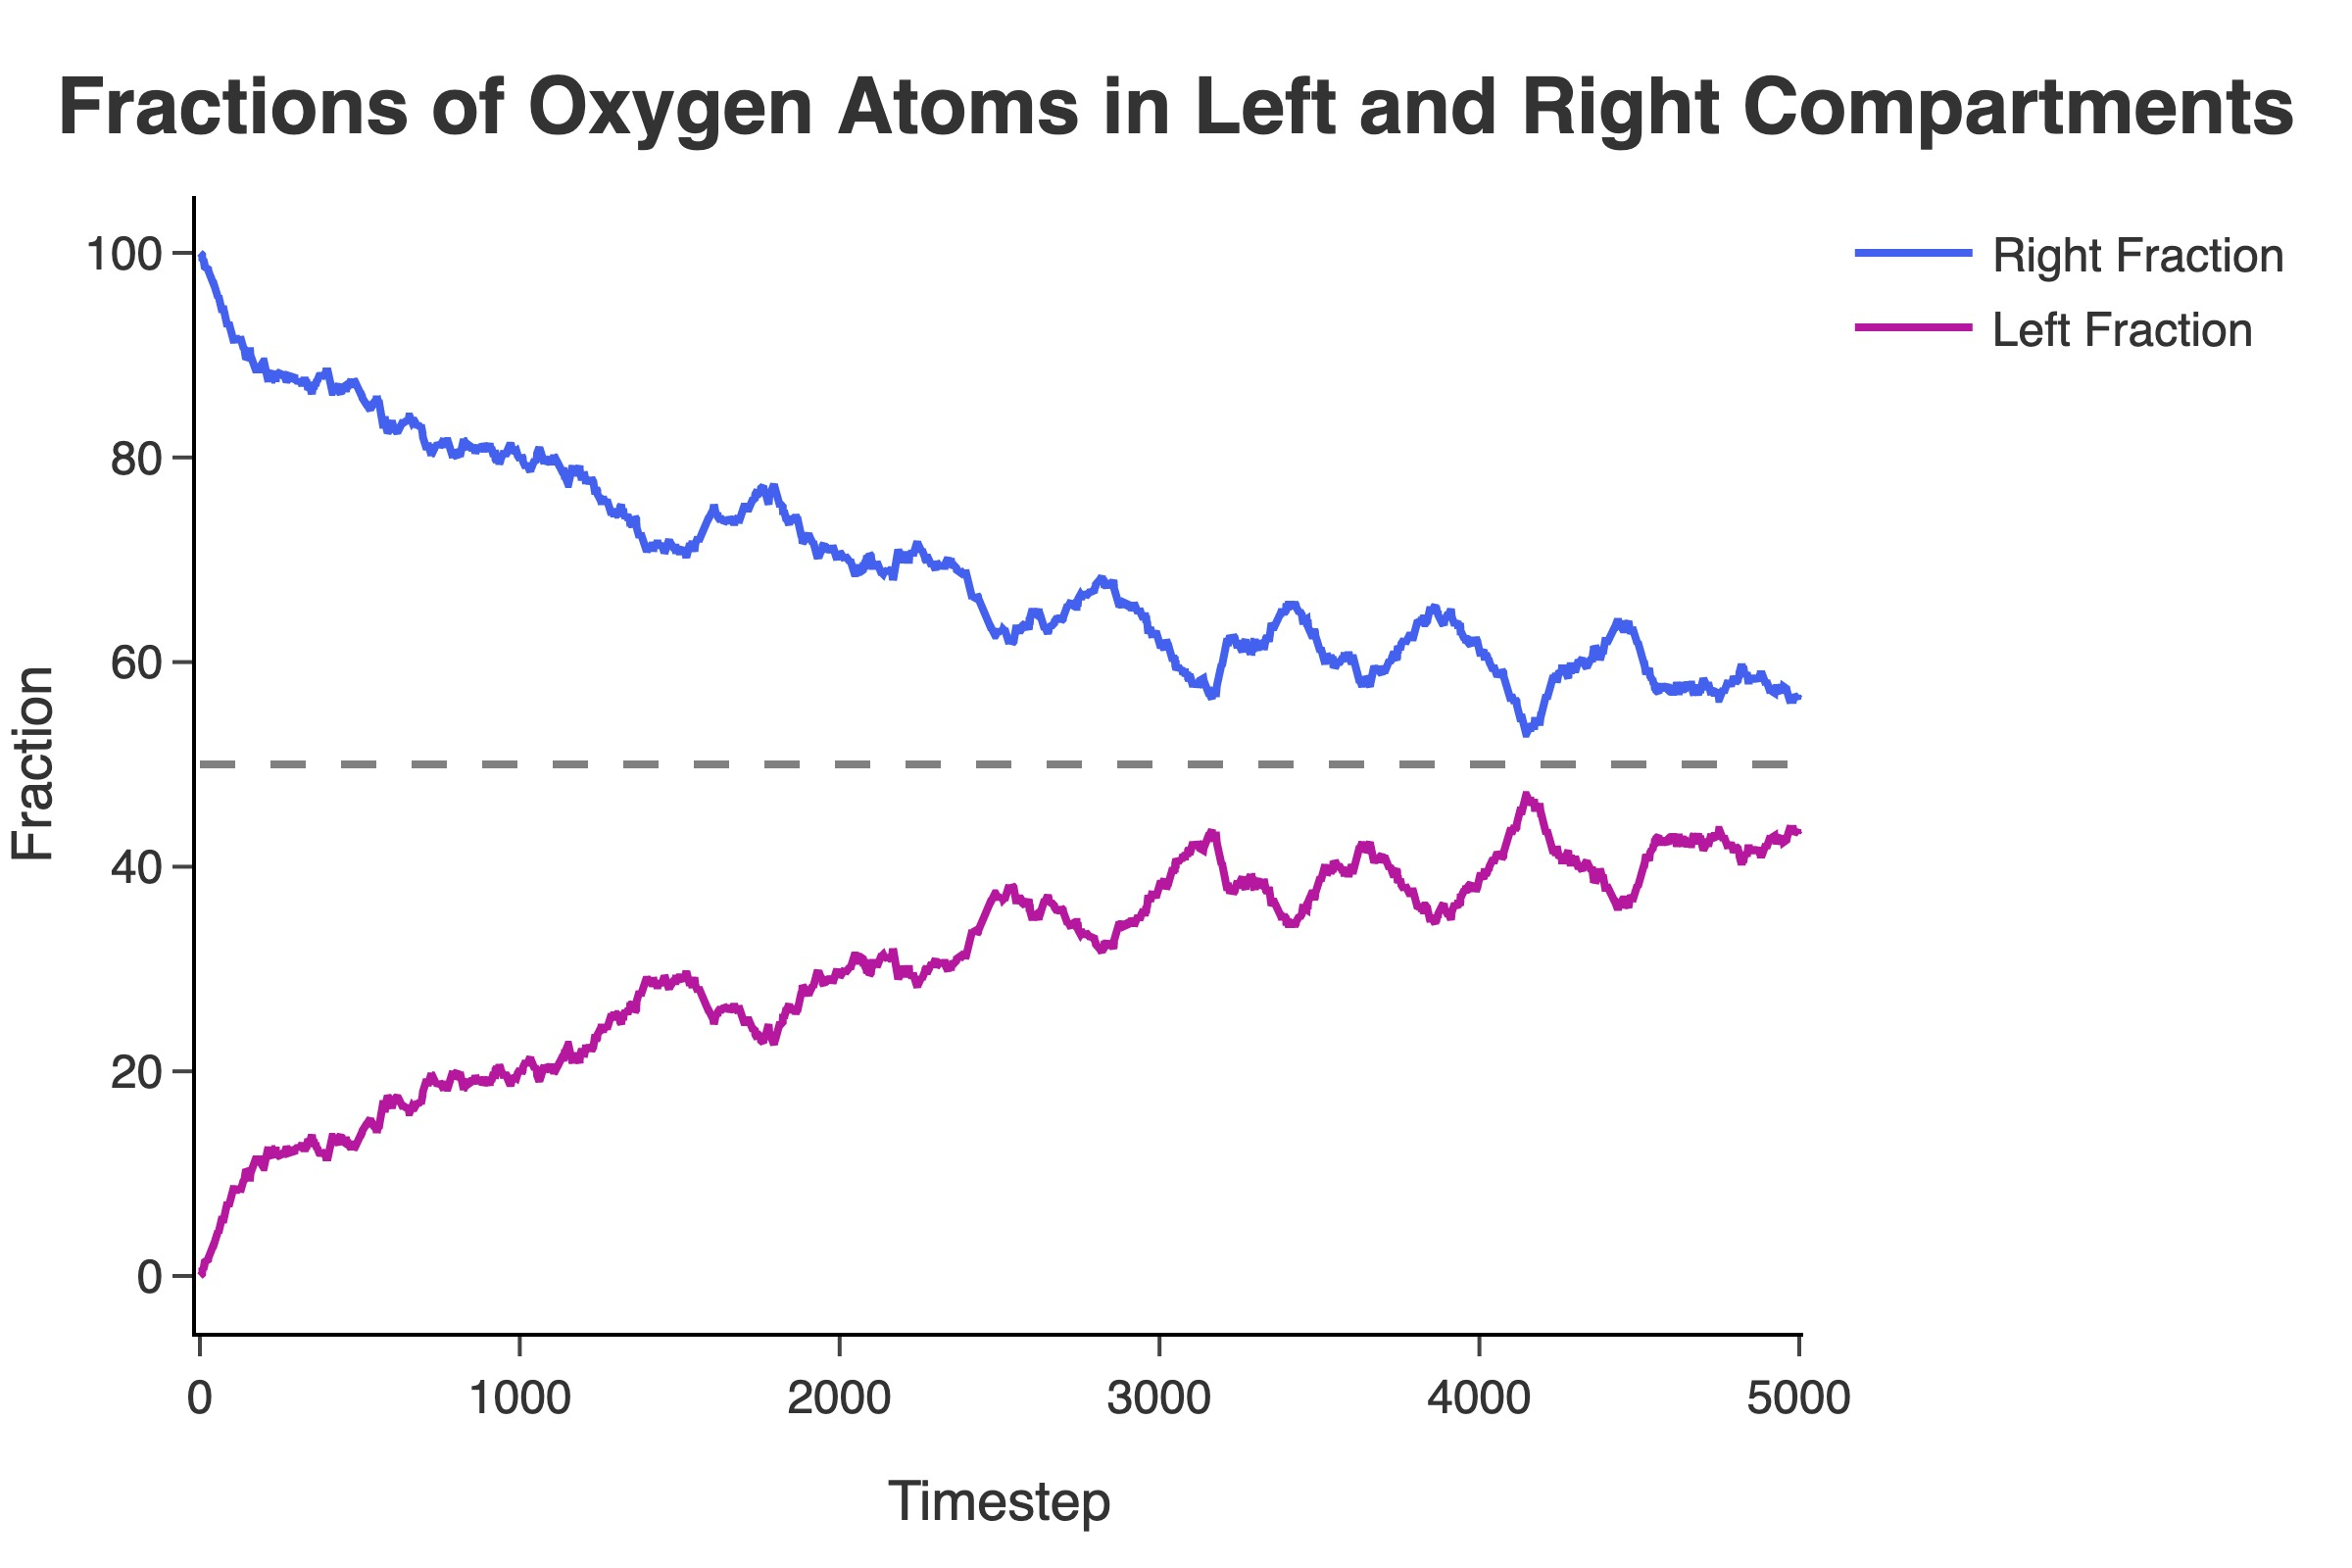
\includegraphics[width=\linewidth]{../figures/jpg/distribution/atoms_1000_temp_5000_compartment_fractions.jpg}
    \end{minipage}
    \begin{minipage}{0.43\linewidth}
        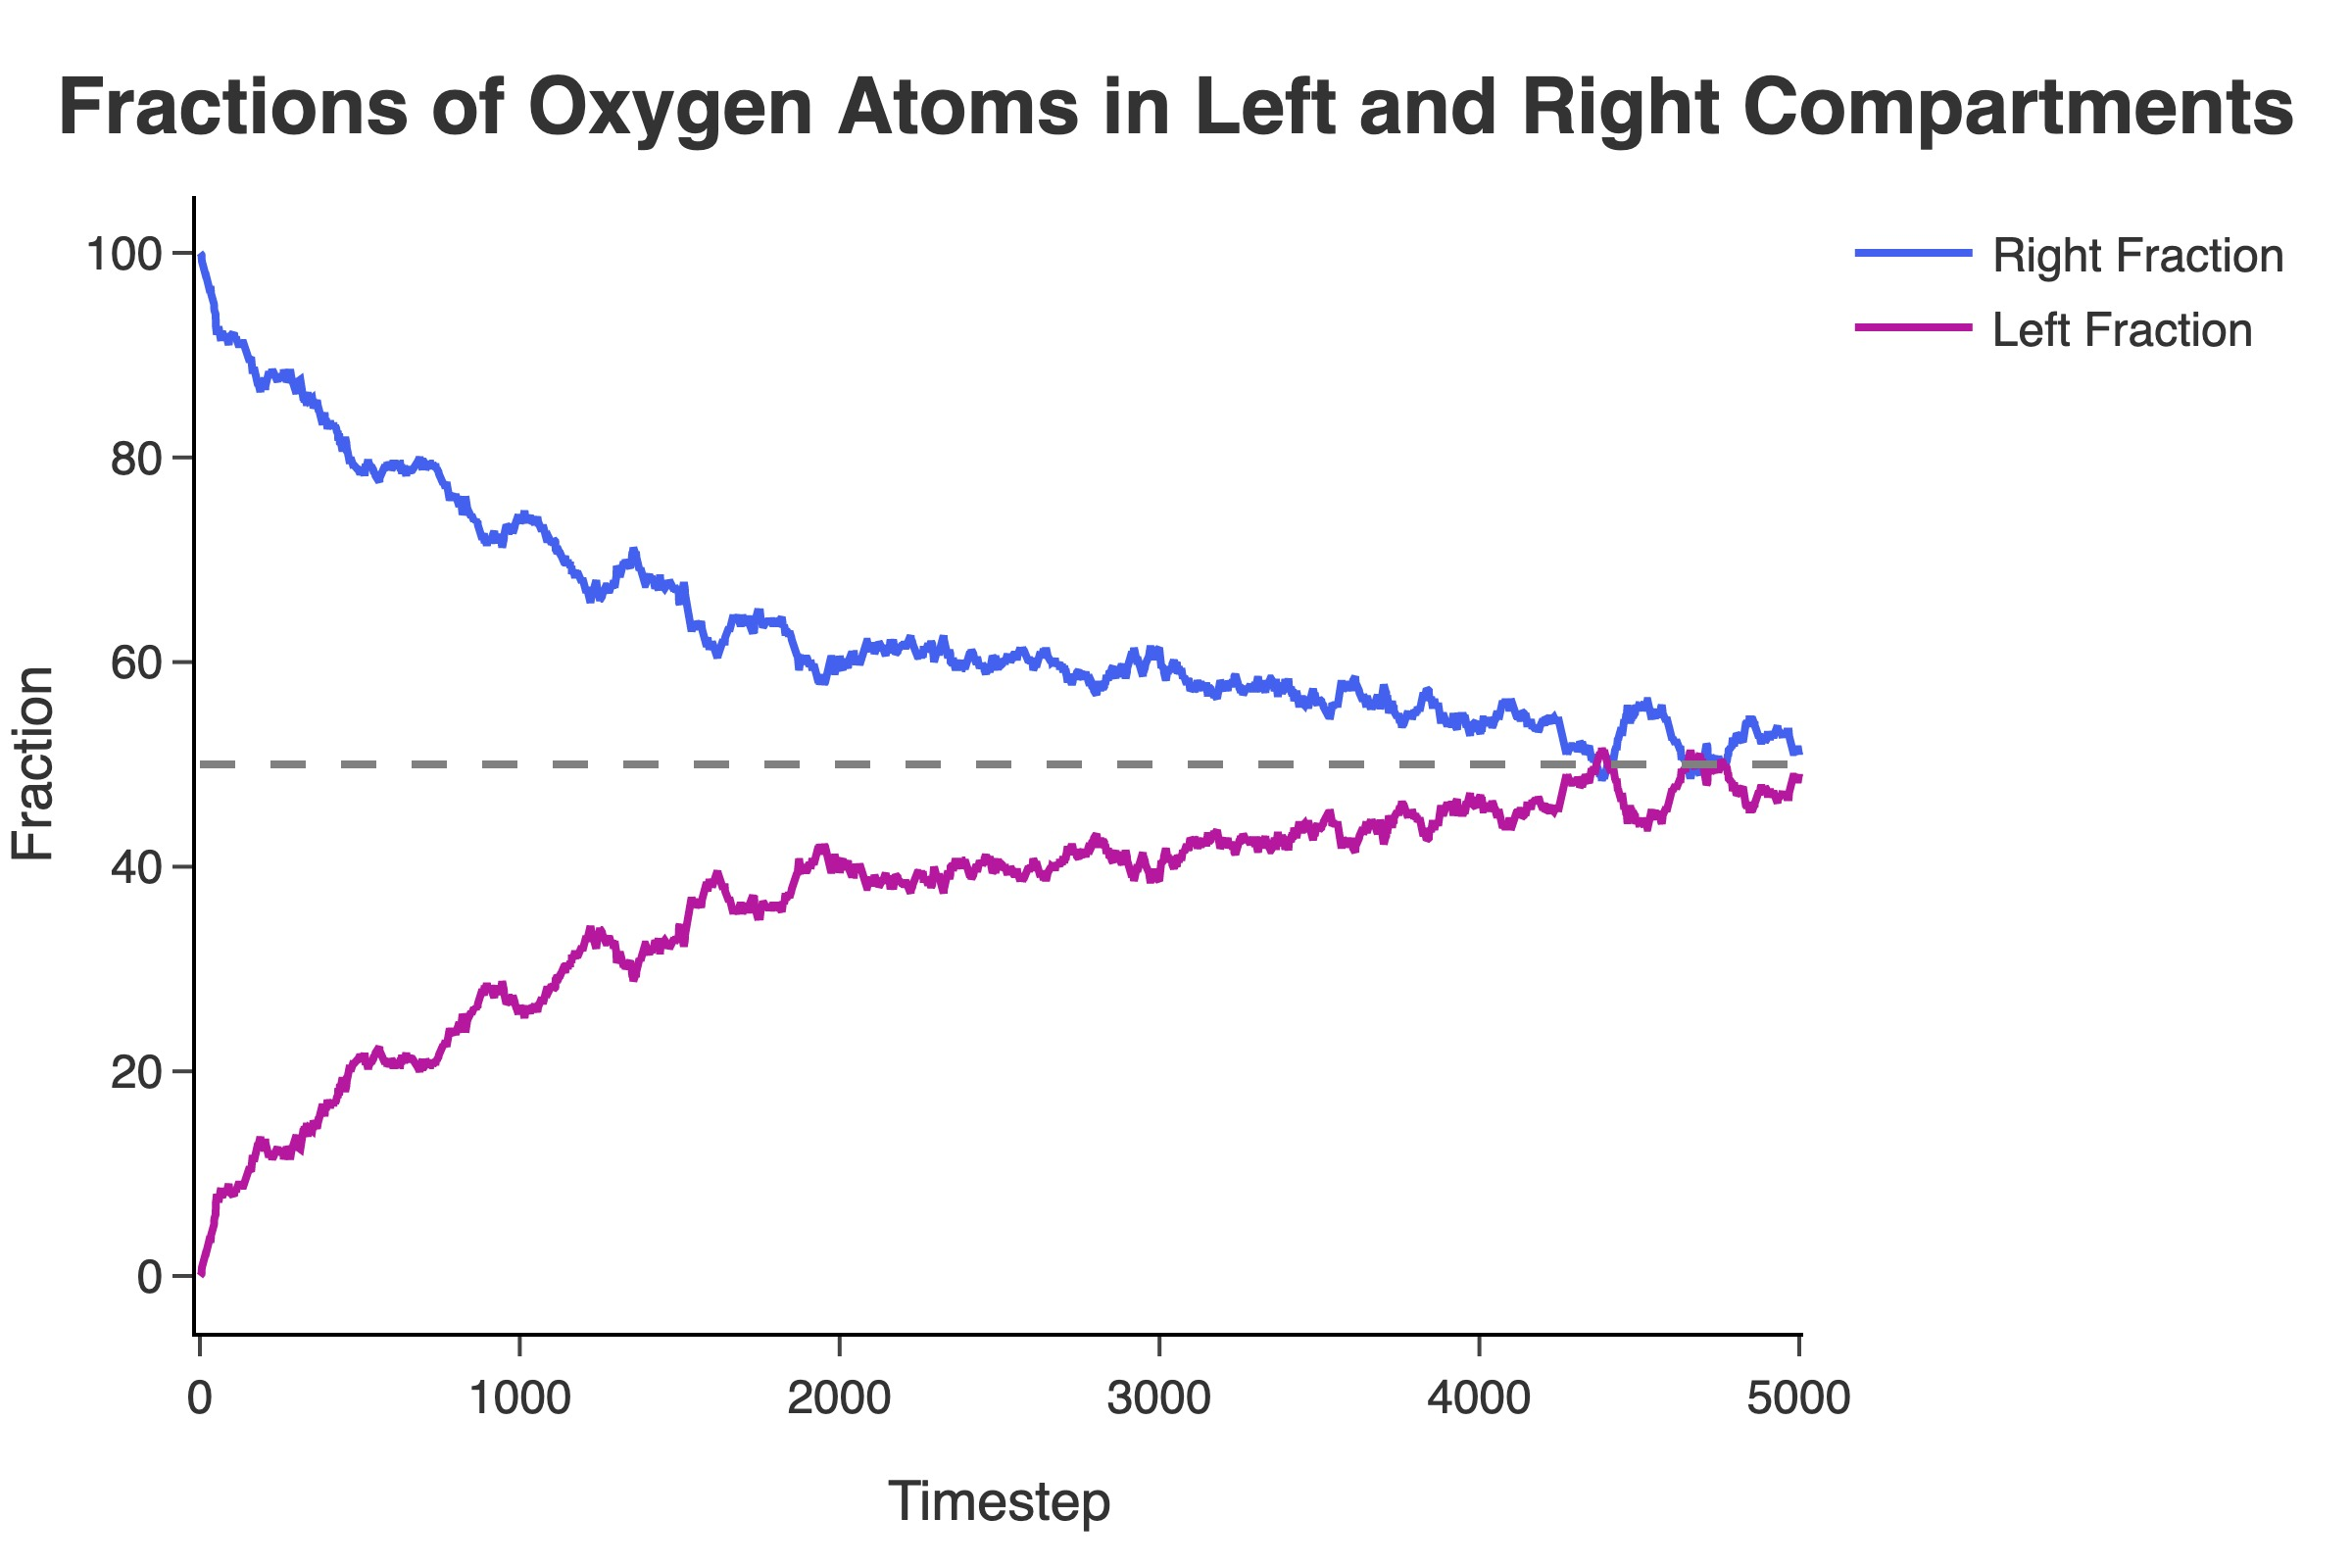
\includegraphics[width=\linewidth]{../figures/jpg/distribution/atoms_1000_temp_10000_compartment_fractions.jpg}
    \end{minipage}
    \caption{Distribution of oxygen atoms in left and right compartments of the closed box as a function of time. Initially, all 1000 oxygen atoms are placed in the right compartment, and the left compartment is filled with 1000 carbon atoms at the same temperature.}
    \label{fig:compartment_fractions}
\end{figure}

\begin{figure}[H]
    \centering
    \begin{minipage}{0.43\linewidth}
        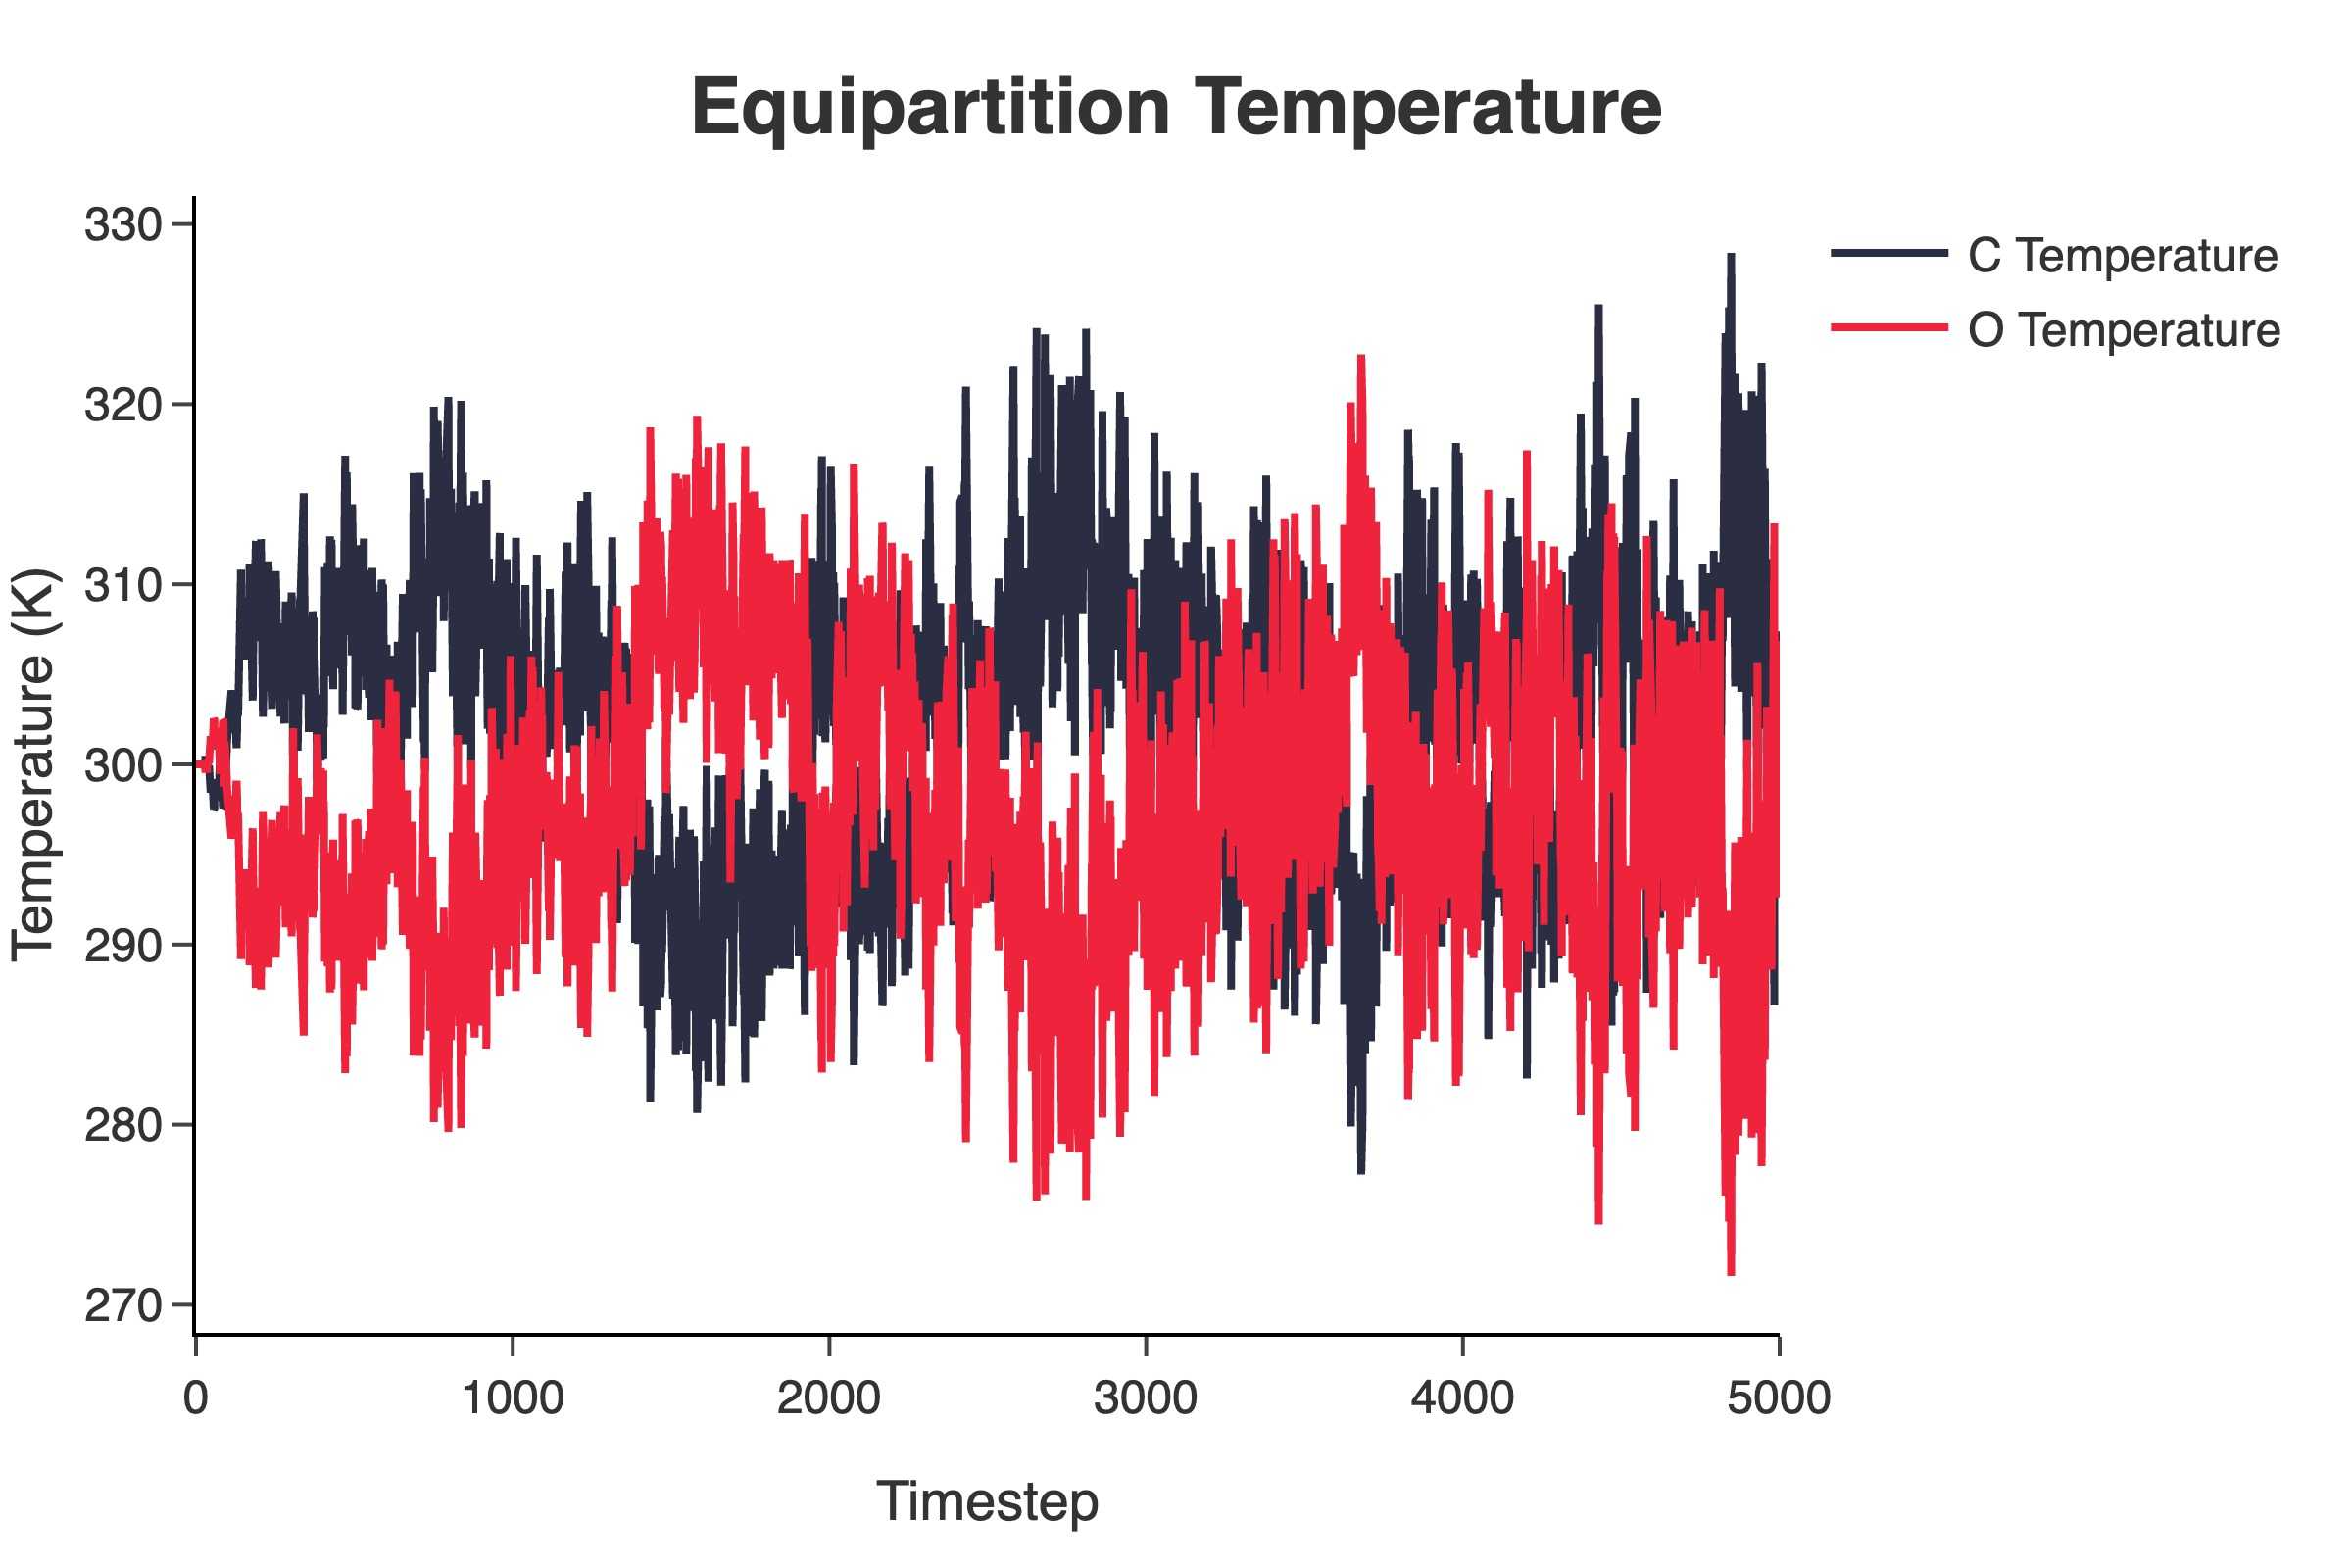
\includegraphics[width=\linewidth]{../figures/jpg/temperature/atoms_1000_temp_300_equipartition_temperature.jpg}
    \end{minipage}
    \begin{minipage}{0.43\linewidth}
        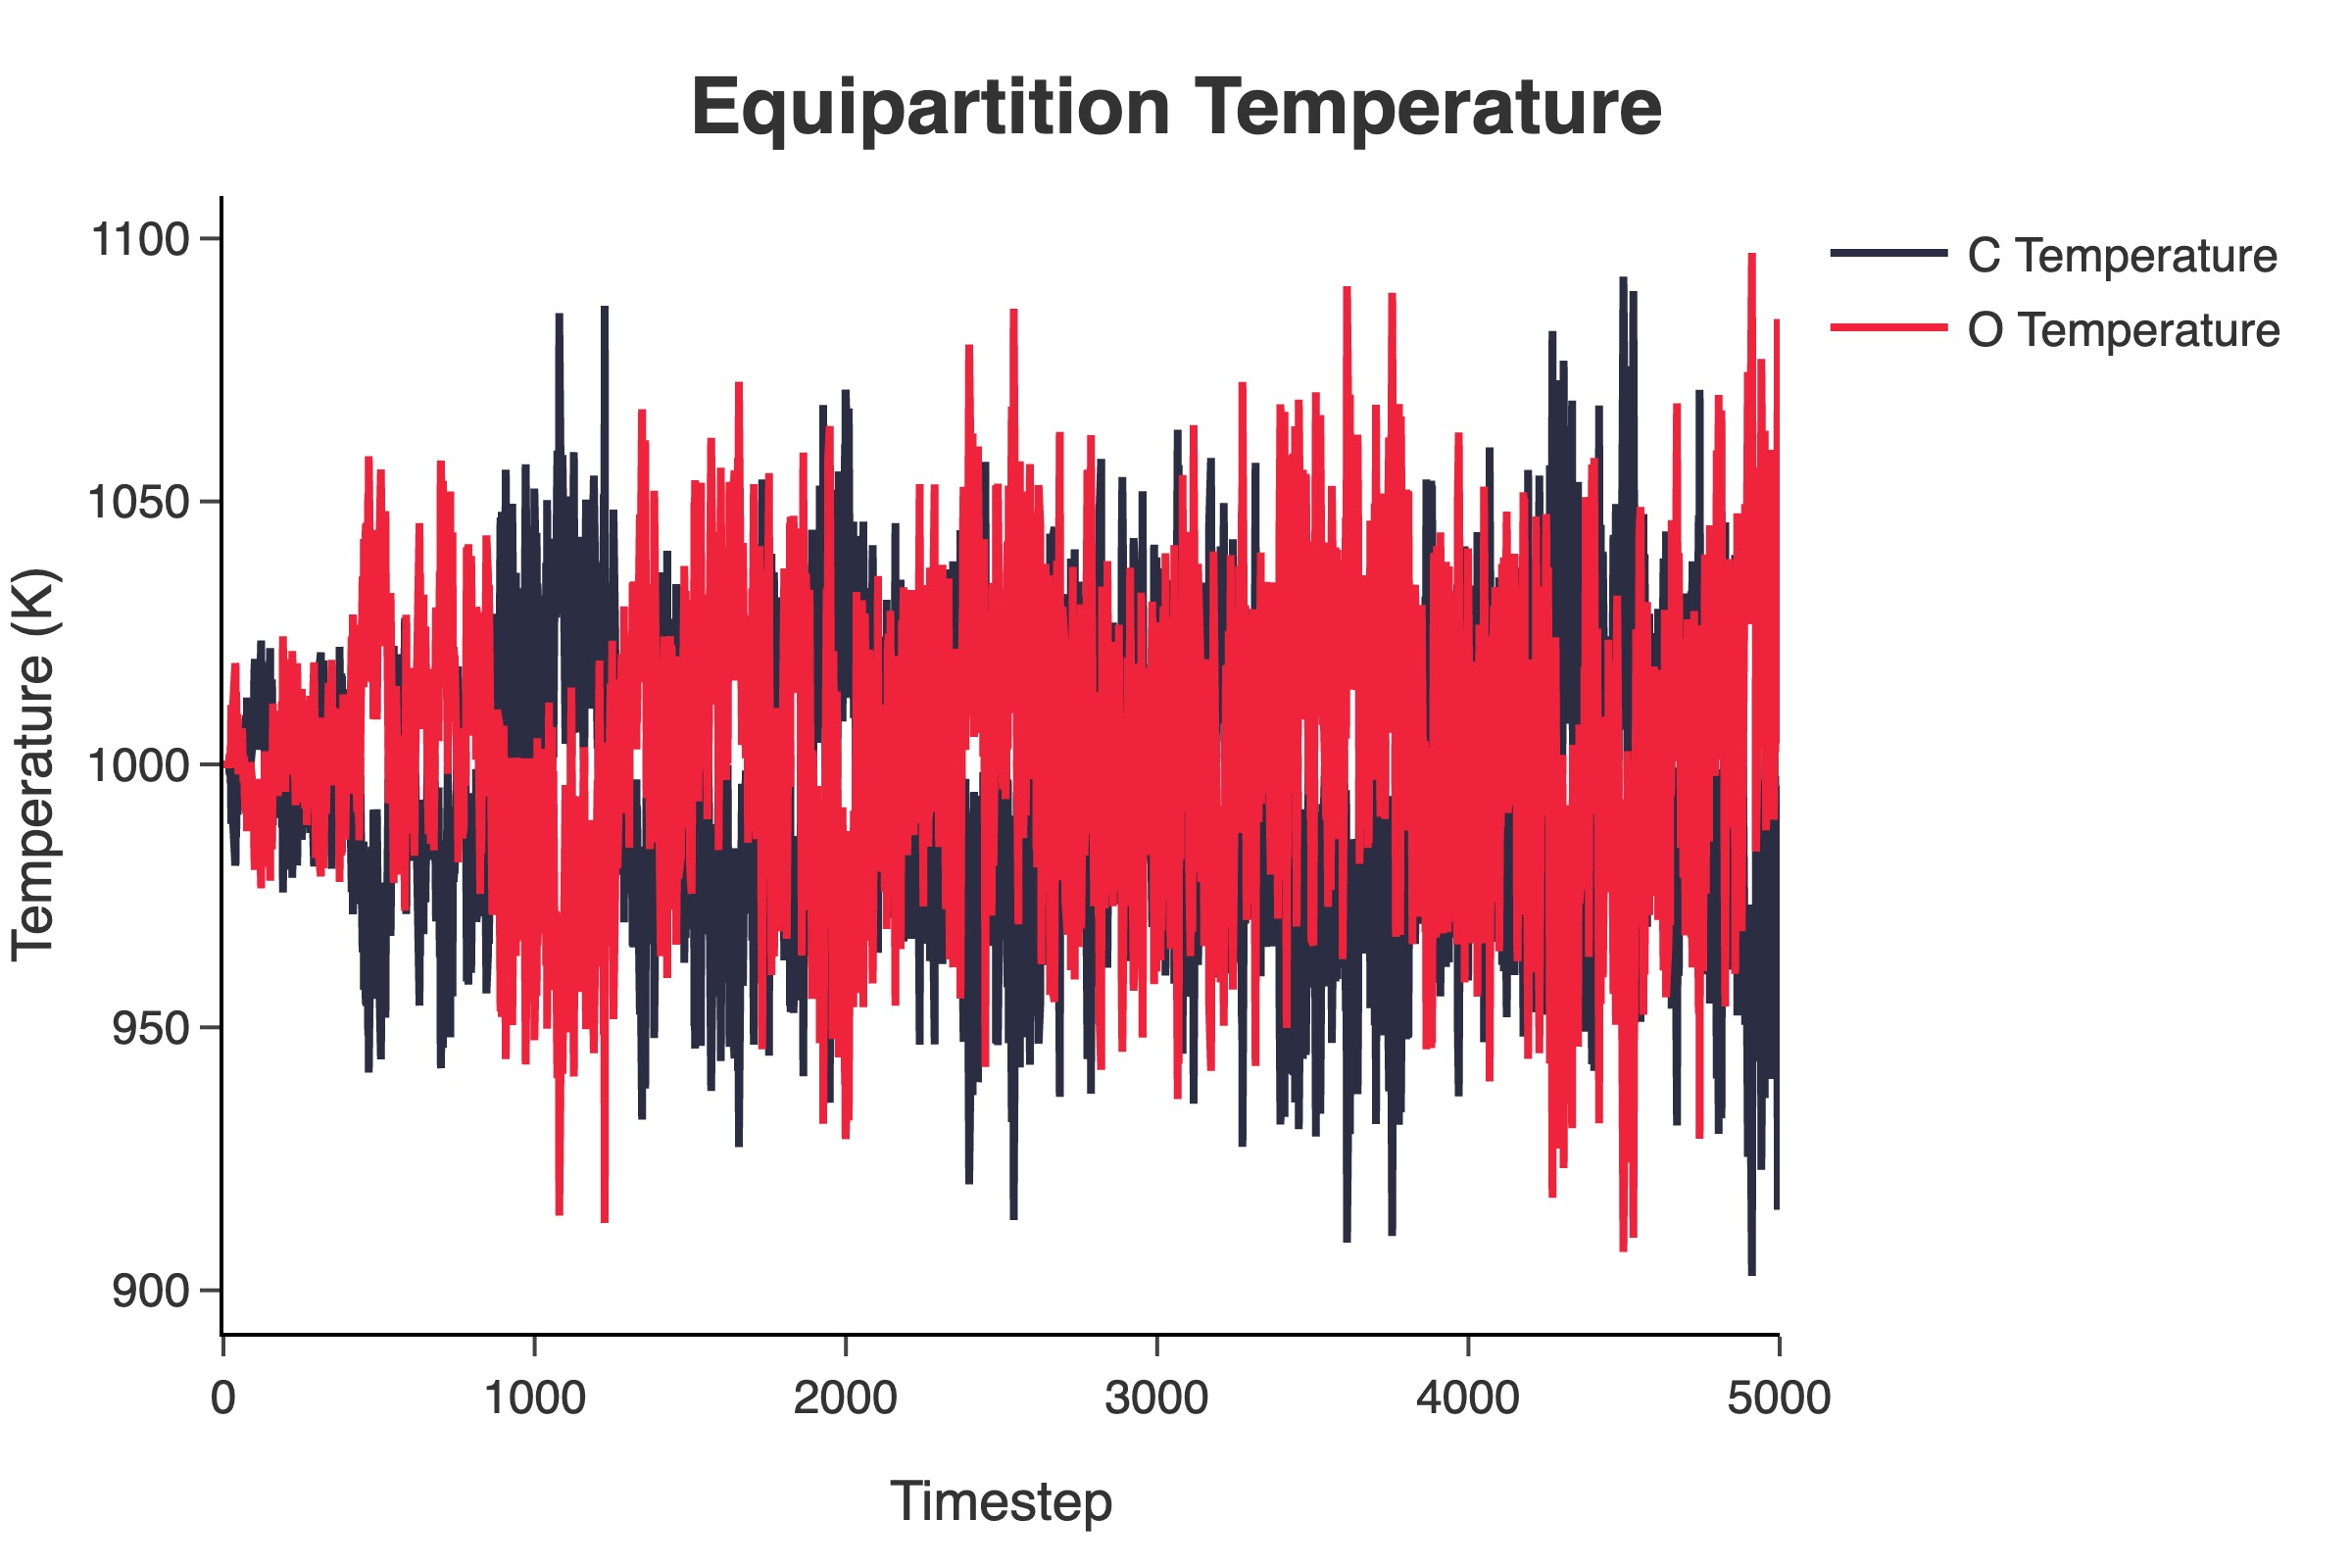
\includegraphics[width=\linewidth]{../figures/jpg/temperature/atoms_1000_temp_1000_equipartition_temperature.jpg}
    \end{minipage} \\
    \begin{minipage}{0.43\linewidth}
        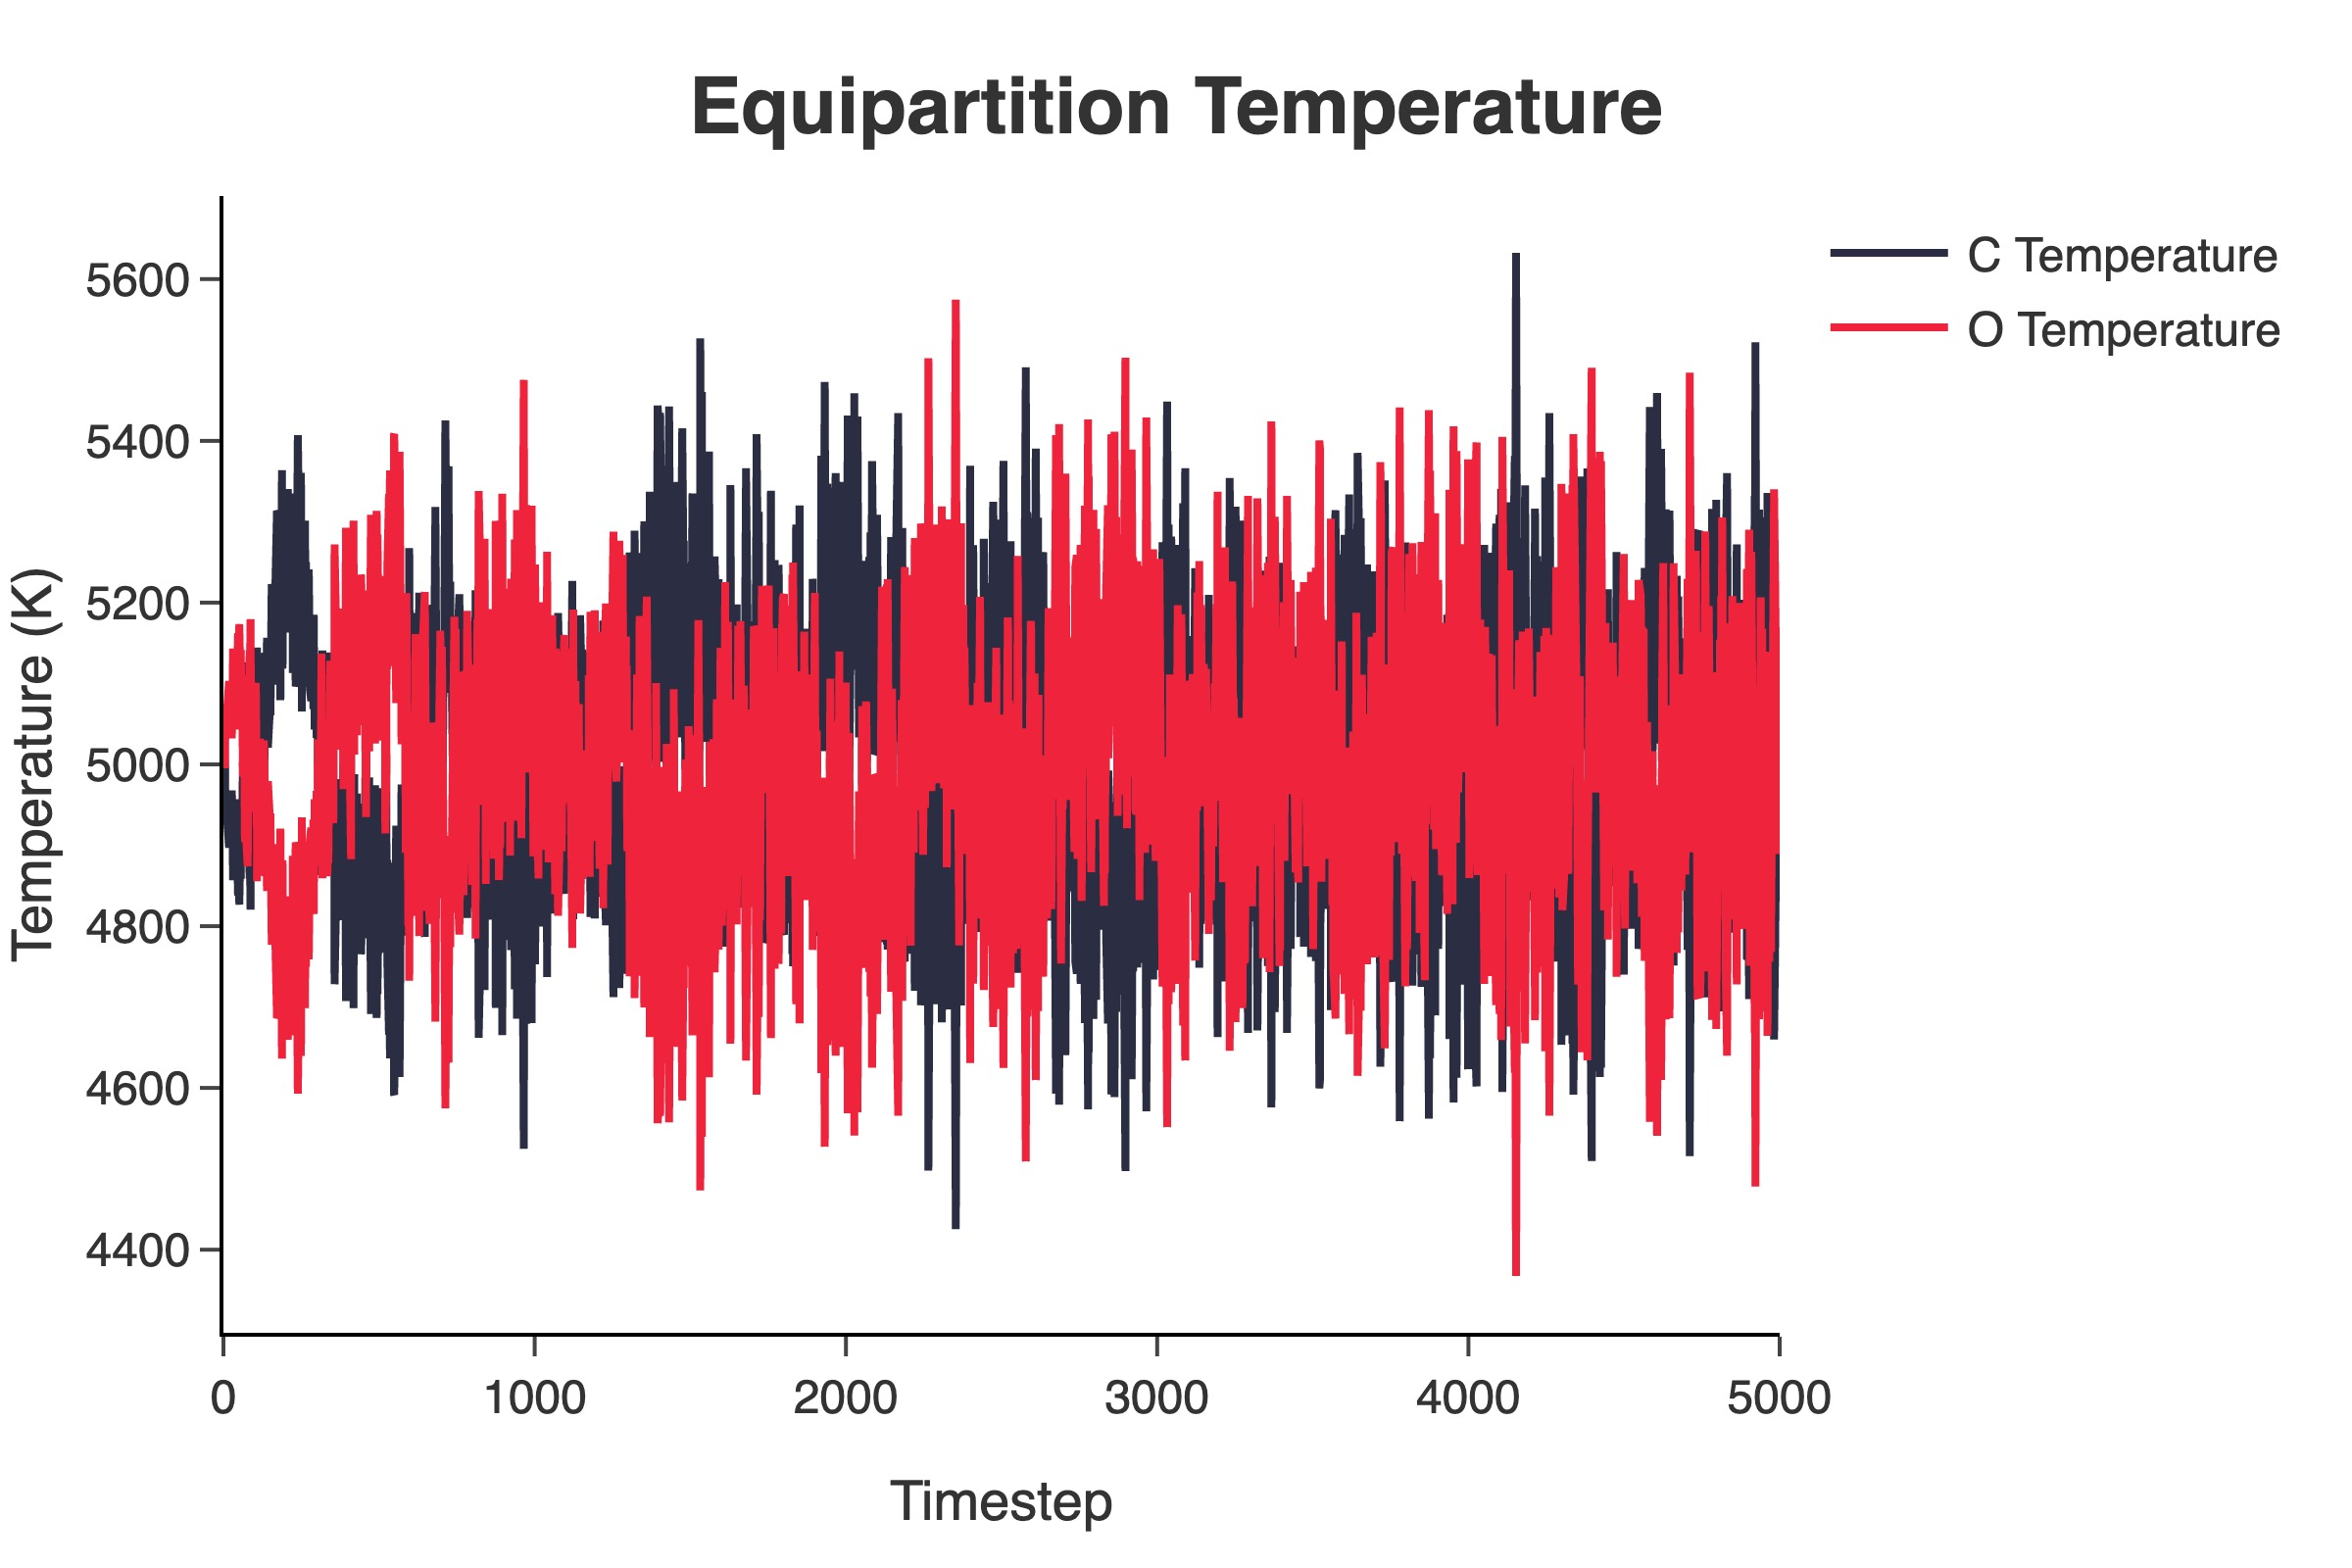
\includegraphics[width=\linewidth]{../figures/jpg/temperature/atoms_1000_temp_5000_equipartition_temperature.jpg}
    \end{minipage}
    \begin{minipage}{0.43\linewidth}
        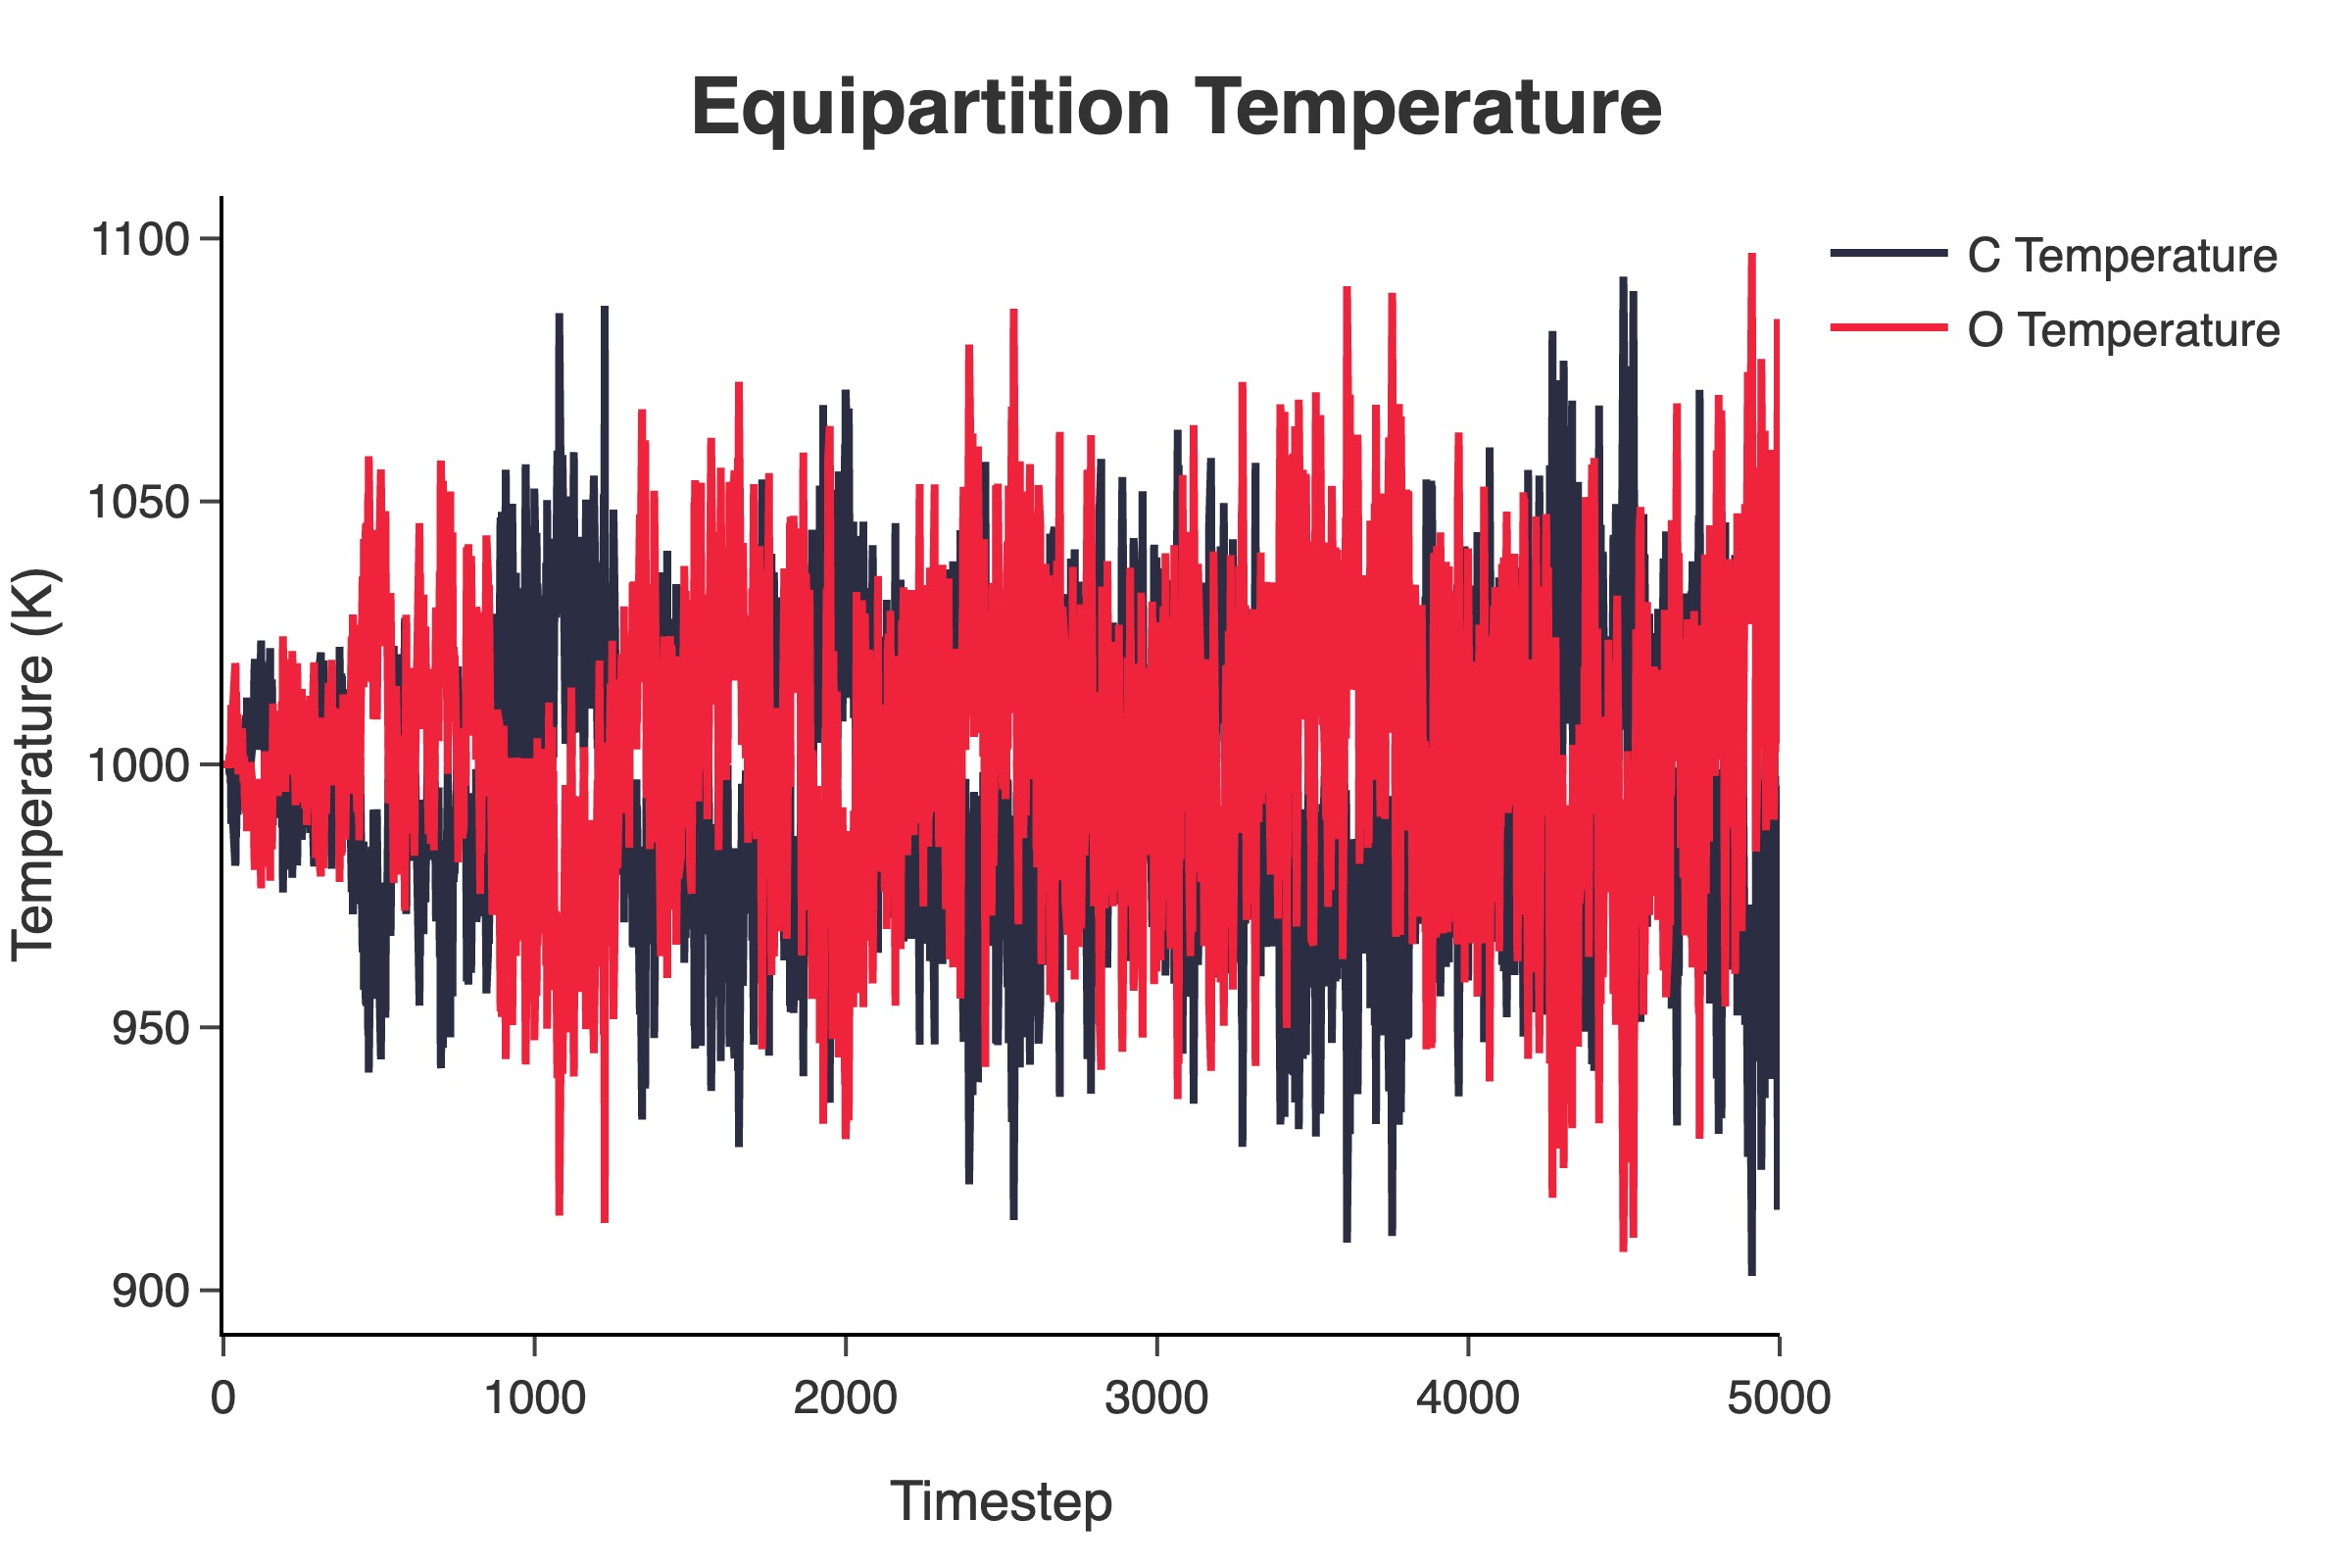
\includegraphics[width=\linewidth]{../figures/jpg/temperature/atoms_1000_temp_1000_equipartition_temperature.jpg}
    \end{minipage}
    \caption{Equipartition temperature of carbon and oxygen atoms (1000 atoms each, initially placed in left and right compartments respectively) as a function of time.}
    \label{fig:temperature_evolution}
\end{figure}

\newpage


\begin{figure}[H]
    \centering
    \begin{minipage}{0.9\linewidth}
        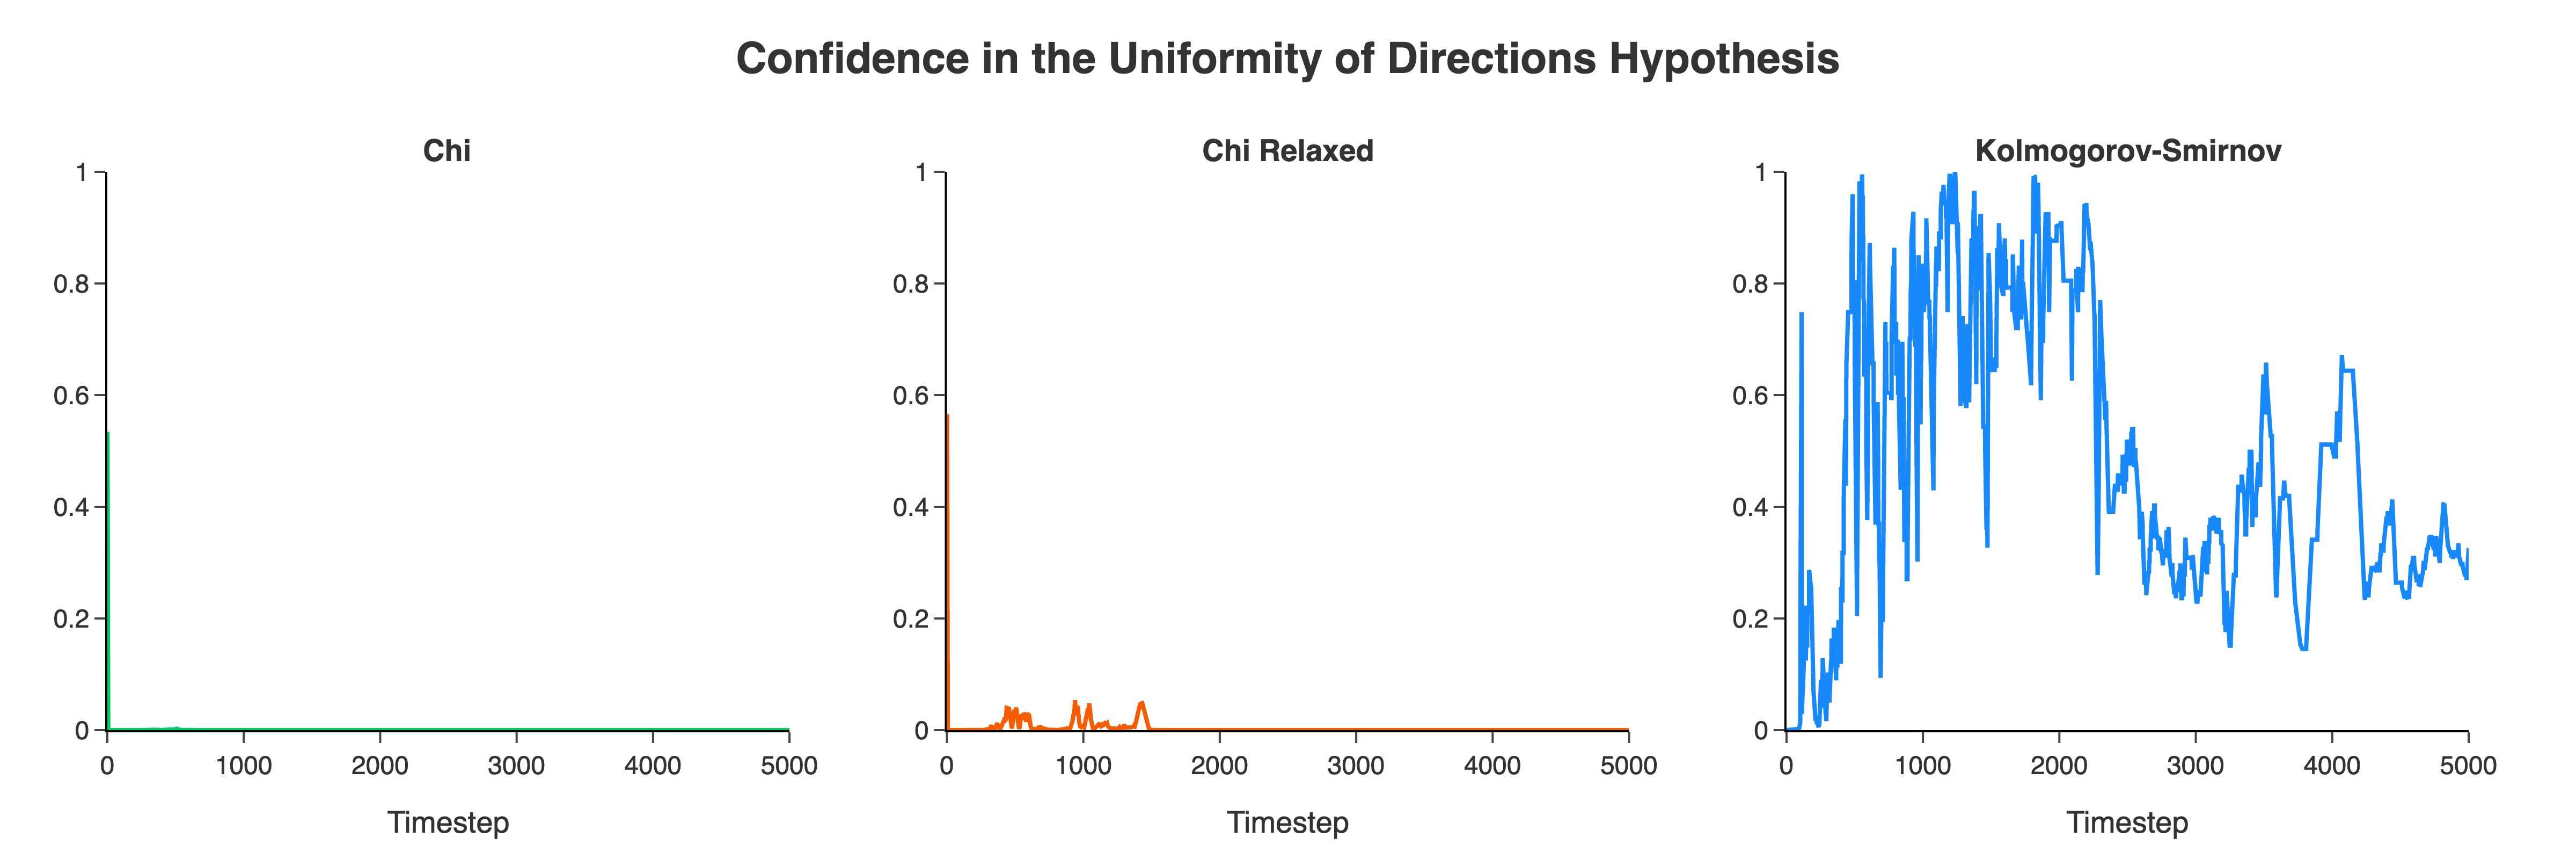
\includegraphics[width=\linewidth]{../figures/jpg/uniformity/atoms_1000_temp_300_uniformity_confidence.jpg}
    \end{minipage} \\
    \begin{minipage}{0.9\linewidth}
        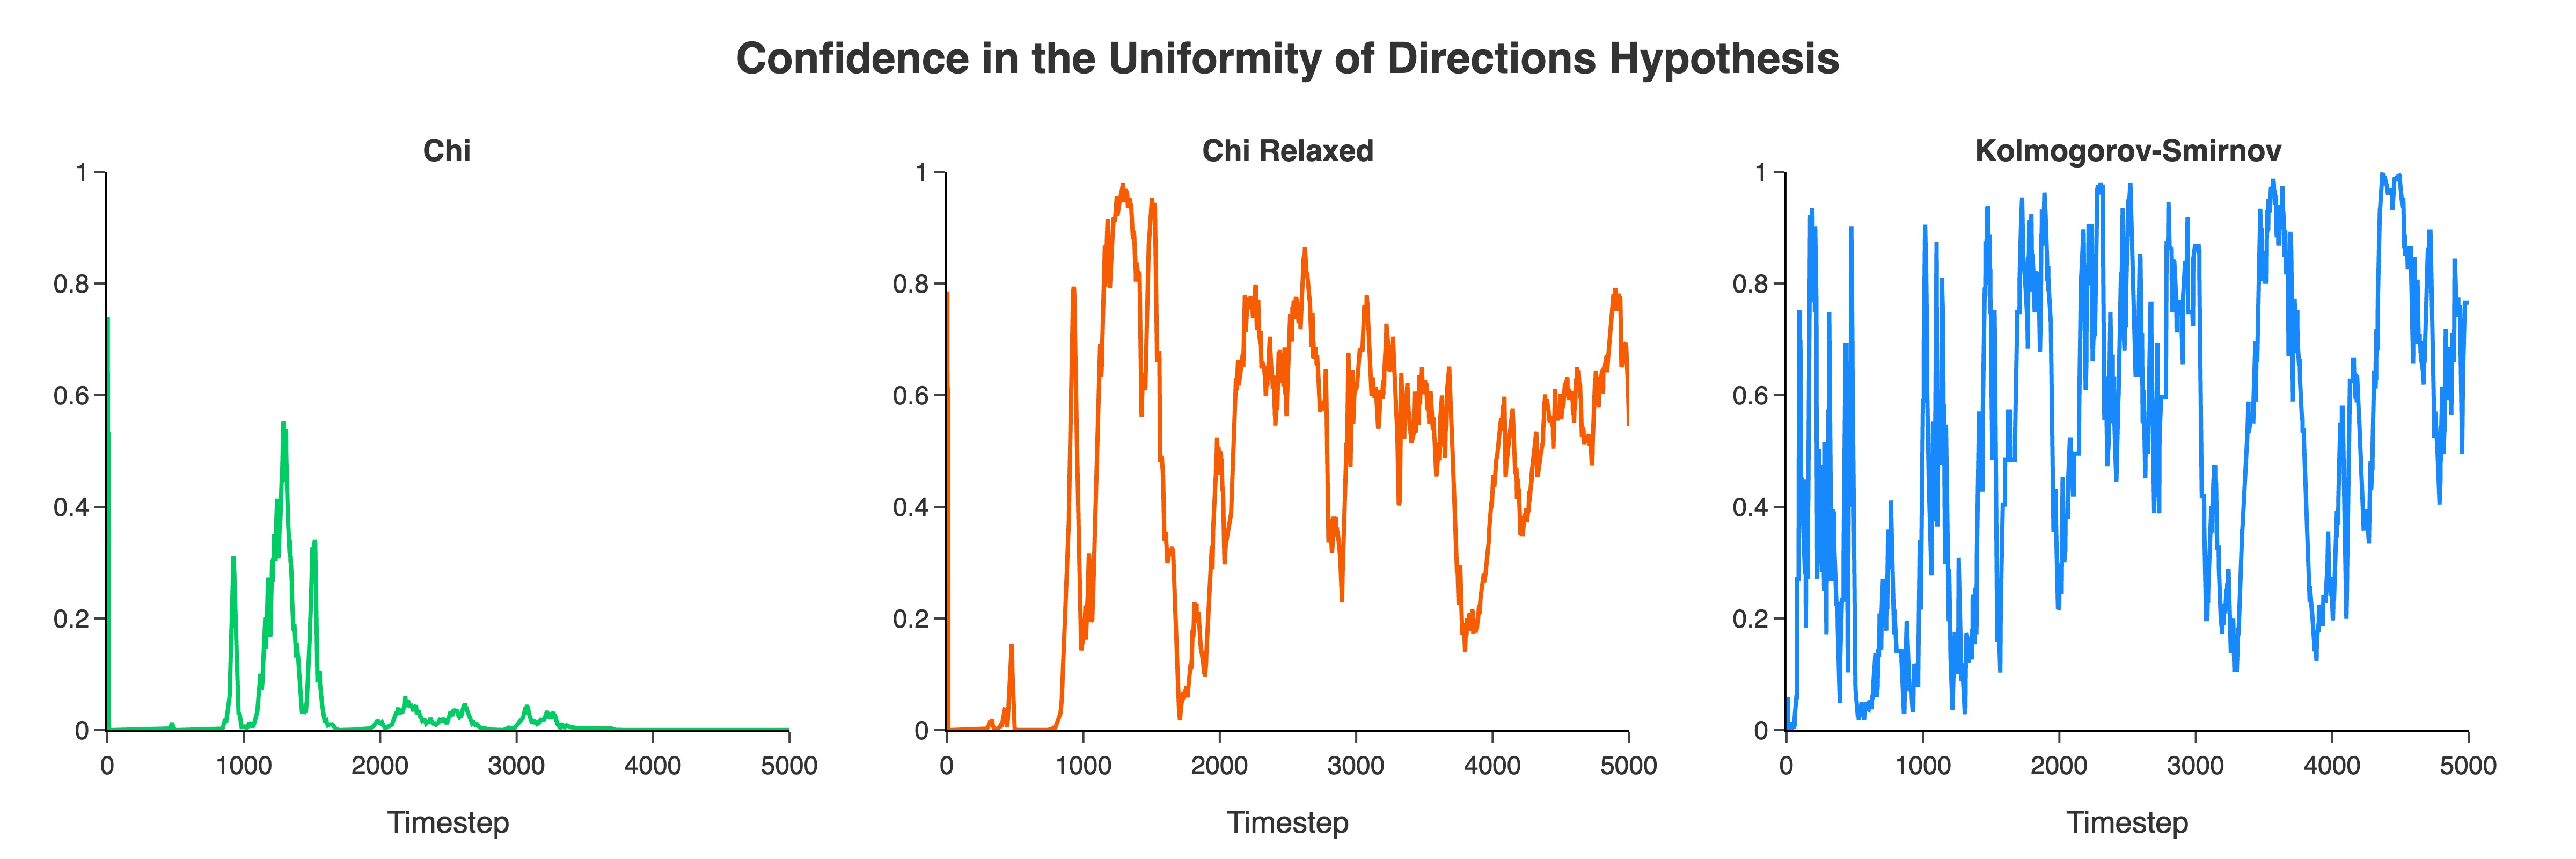
\includegraphics[width=\linewidth]{../figures/jpg/uniformity/atoms_1000_temp_1000_uniformity_confidence.jpg}
    \end{minipage} \\
    \begin{minipage}{0.9\linewidth}
        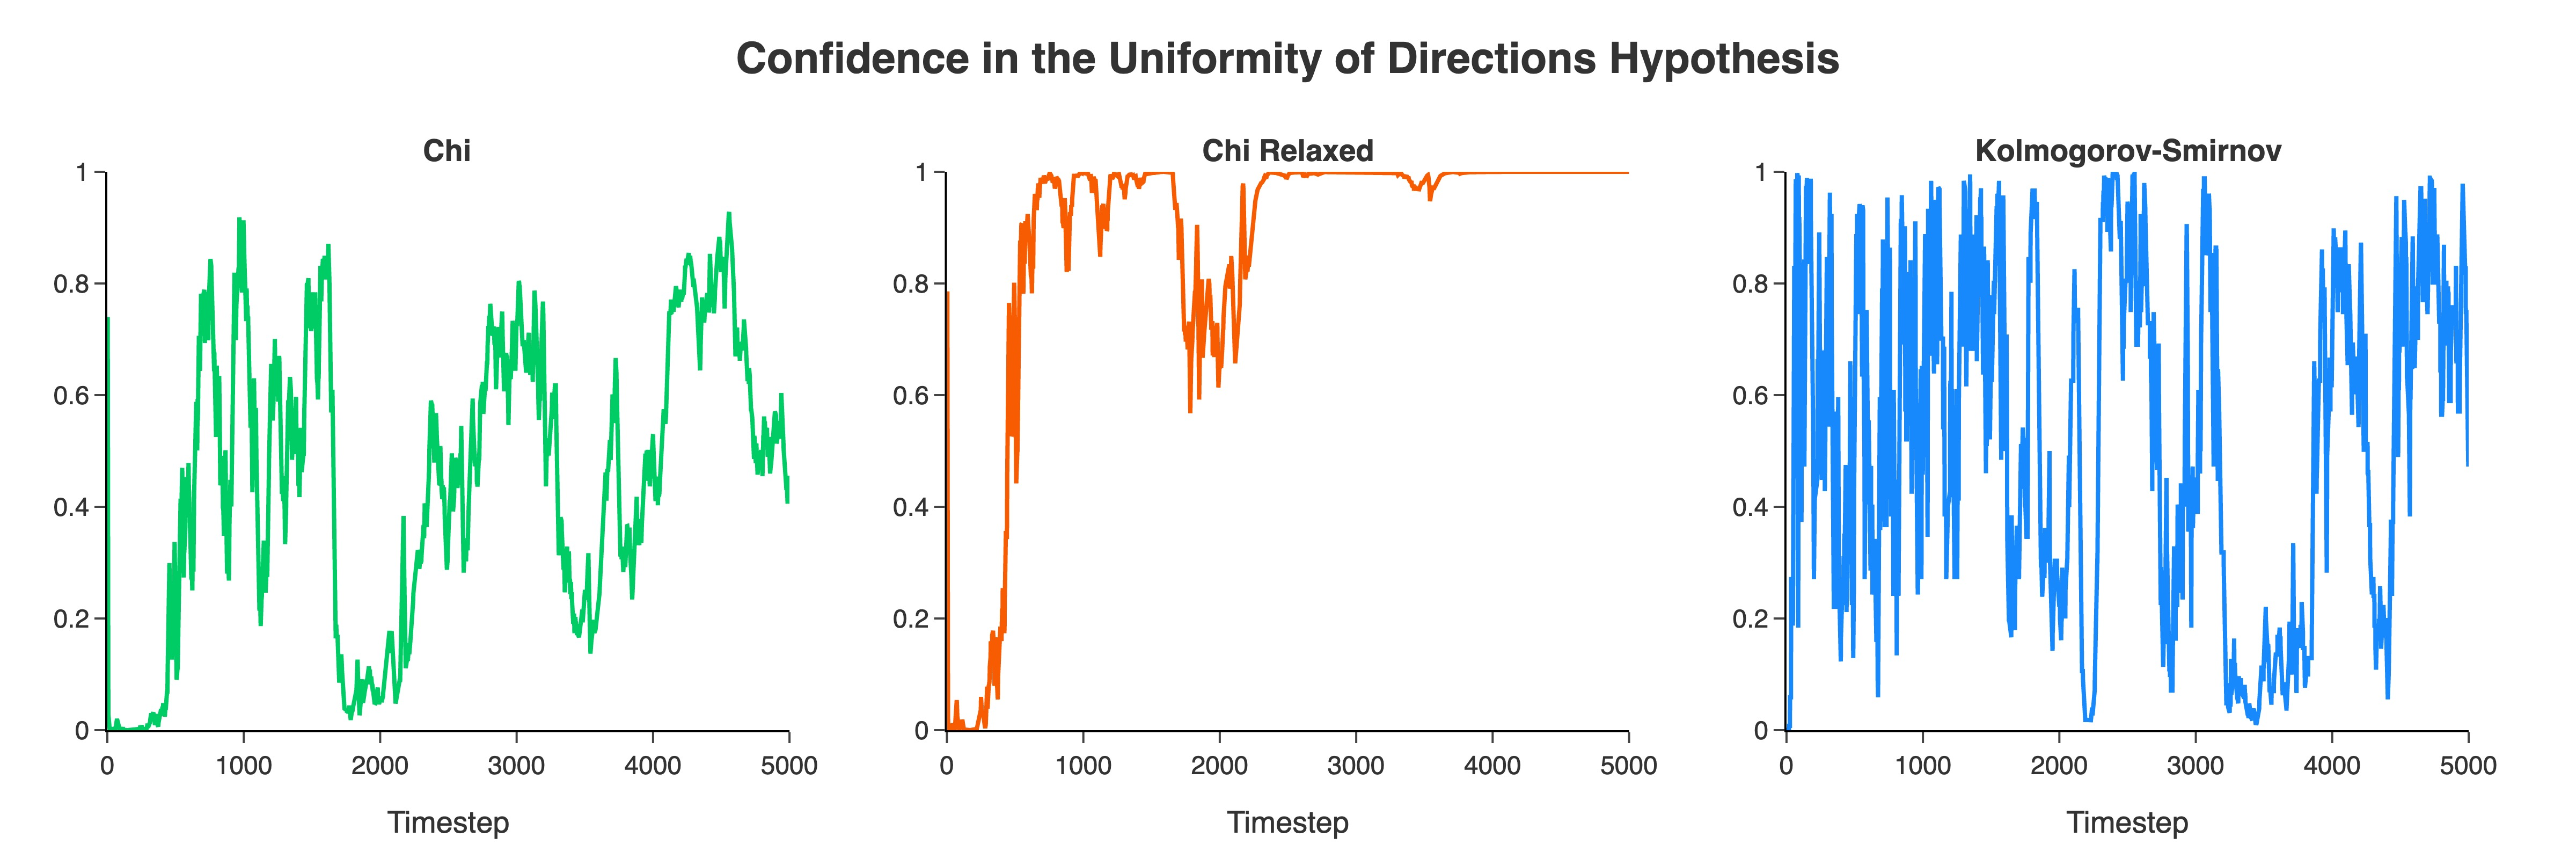
\includegraphics[width=\linewidth]{../figures/jpg/uniformity/atoms_1000_temp_5000_uniformity_confidence.jpg}
    \end{minipage} \\
    \begin{minipage}{0.9\linewidth}
        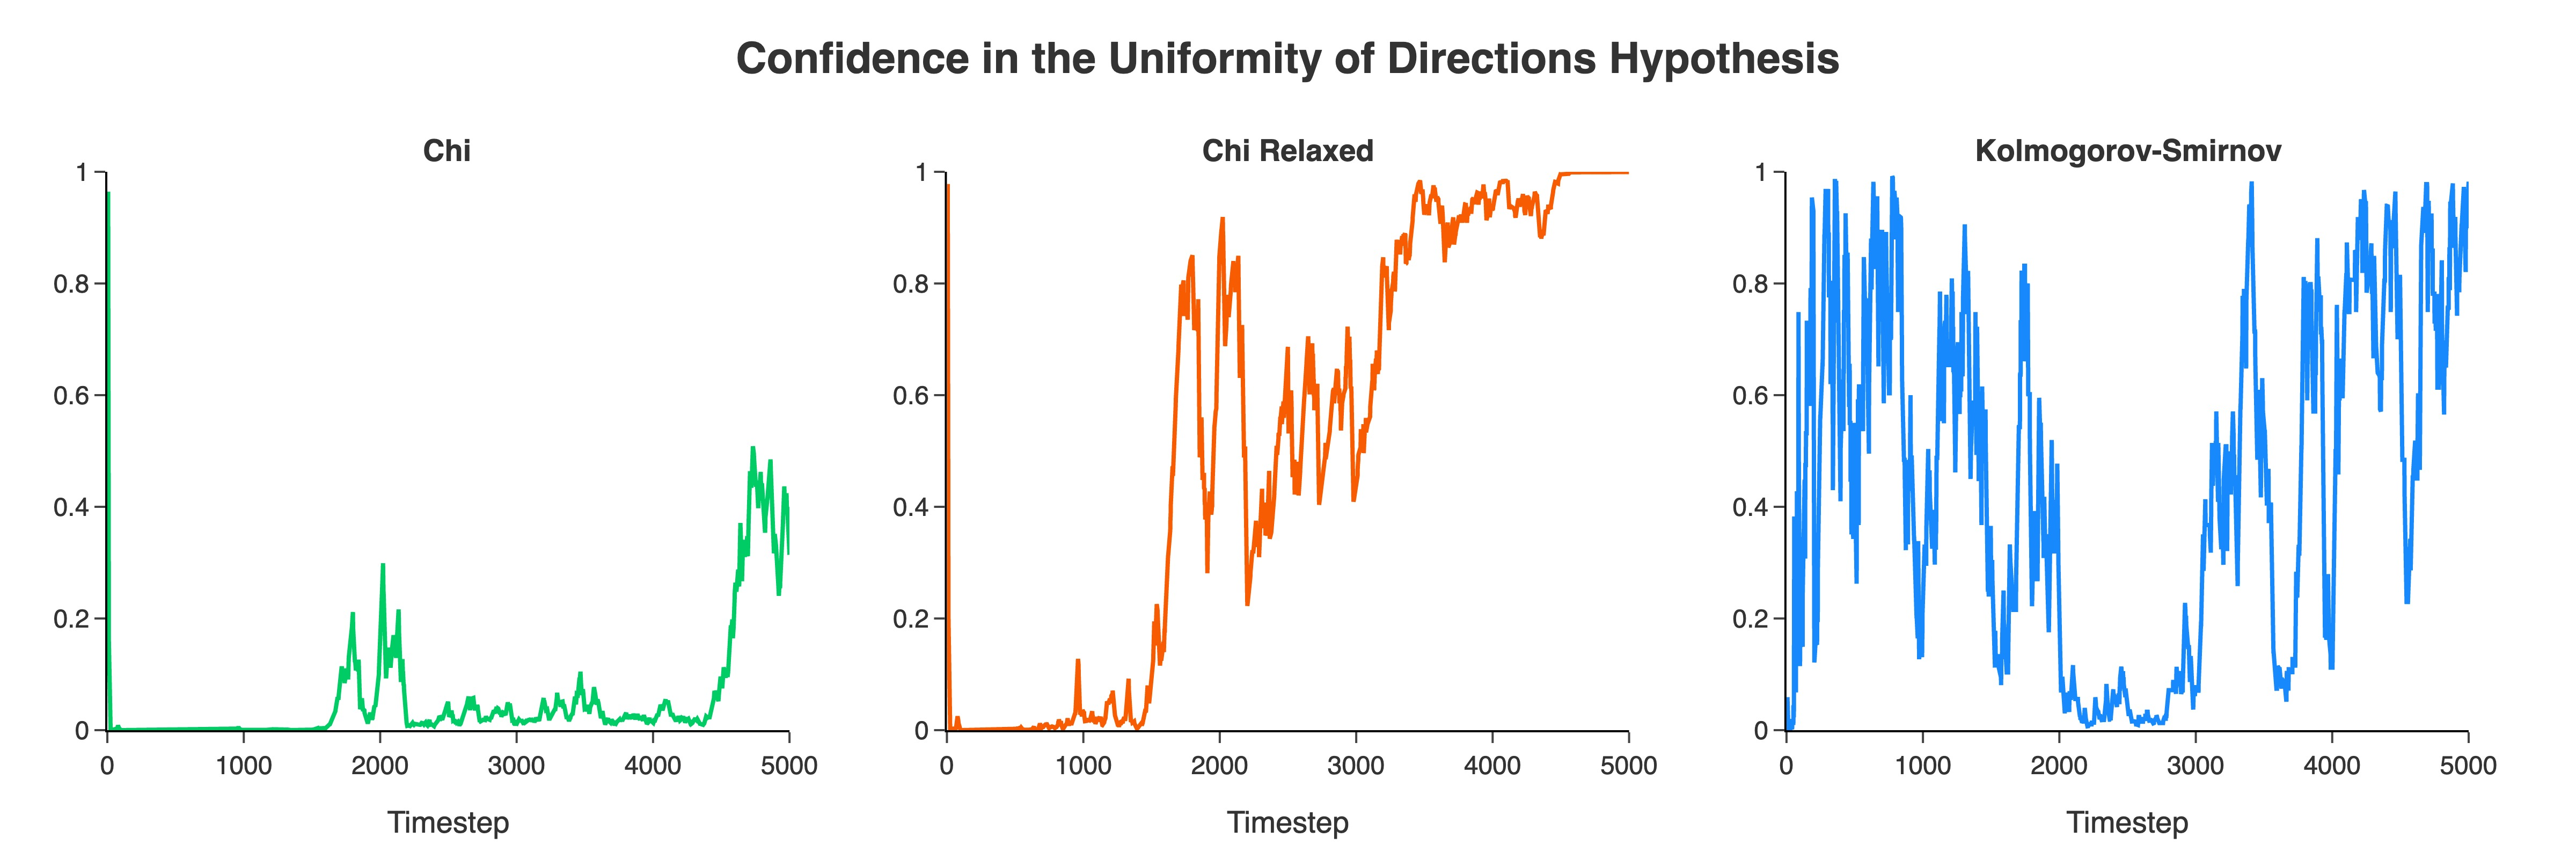
\includegraphics[width=\linewidth]{../figures/jpg/uniformity/atoms_1000_temp_10000_uniformity_confidence.jpg}
    \end{minipage}
    \caption{Evaluation of the uniformity of the distribution of polar angles of velocities of a single particle (the container contains 2000 particles in total). The polar angle is defined as $\theta=\arctan(v_y/v_x)$. The distribution of $\theta$ is expected to be uniform. The plots show the p-values determined by chi-squared, relaxed chi-squared (deviations from uniformity of 5\% and less are not penalized), Kolmogorov-Smirnov statistic as a function of time and a histogram of the distribution of angles $[-3.14, 3.14]$ at the last timestep of the simulation.}
    \label{fig:uniformity_confidence}
\end{figure}

\newpage

\begin{figure}[h]
    \centering
    \includegraphics[width=0.6\linewidth]{../figures/jpg/pvals/last100_pvals.jpg}
    \caption{Average value of p-value determined by relaxed chi-squared (deviations from uniformity of 5\% and less are not penalized) statistic for the last 100 timesteps of the simulation as a function of temperature and the number of particles.}
    \label{fig:uniformity_summary}
\end{figure}


\begin{figure}[h]
    \centering
    \begin{minipage}{0.49\linewidth}
        \includegraphics[width=\linewidth]{../figures/jpg/distribution/2023-12-18 21:42_compartment_fractions.jpg}
    \end{minipage} 
    \begin{minipage}{0.49\linewidth}
        \includegraphics[width=\linewidth]{../figures/jpg/temperature/2023-12-18 21:42_equipartition_temperature.jpg}
    \end{minipage} 
    % \begin{minipage}{0.9\linewidth}
    %     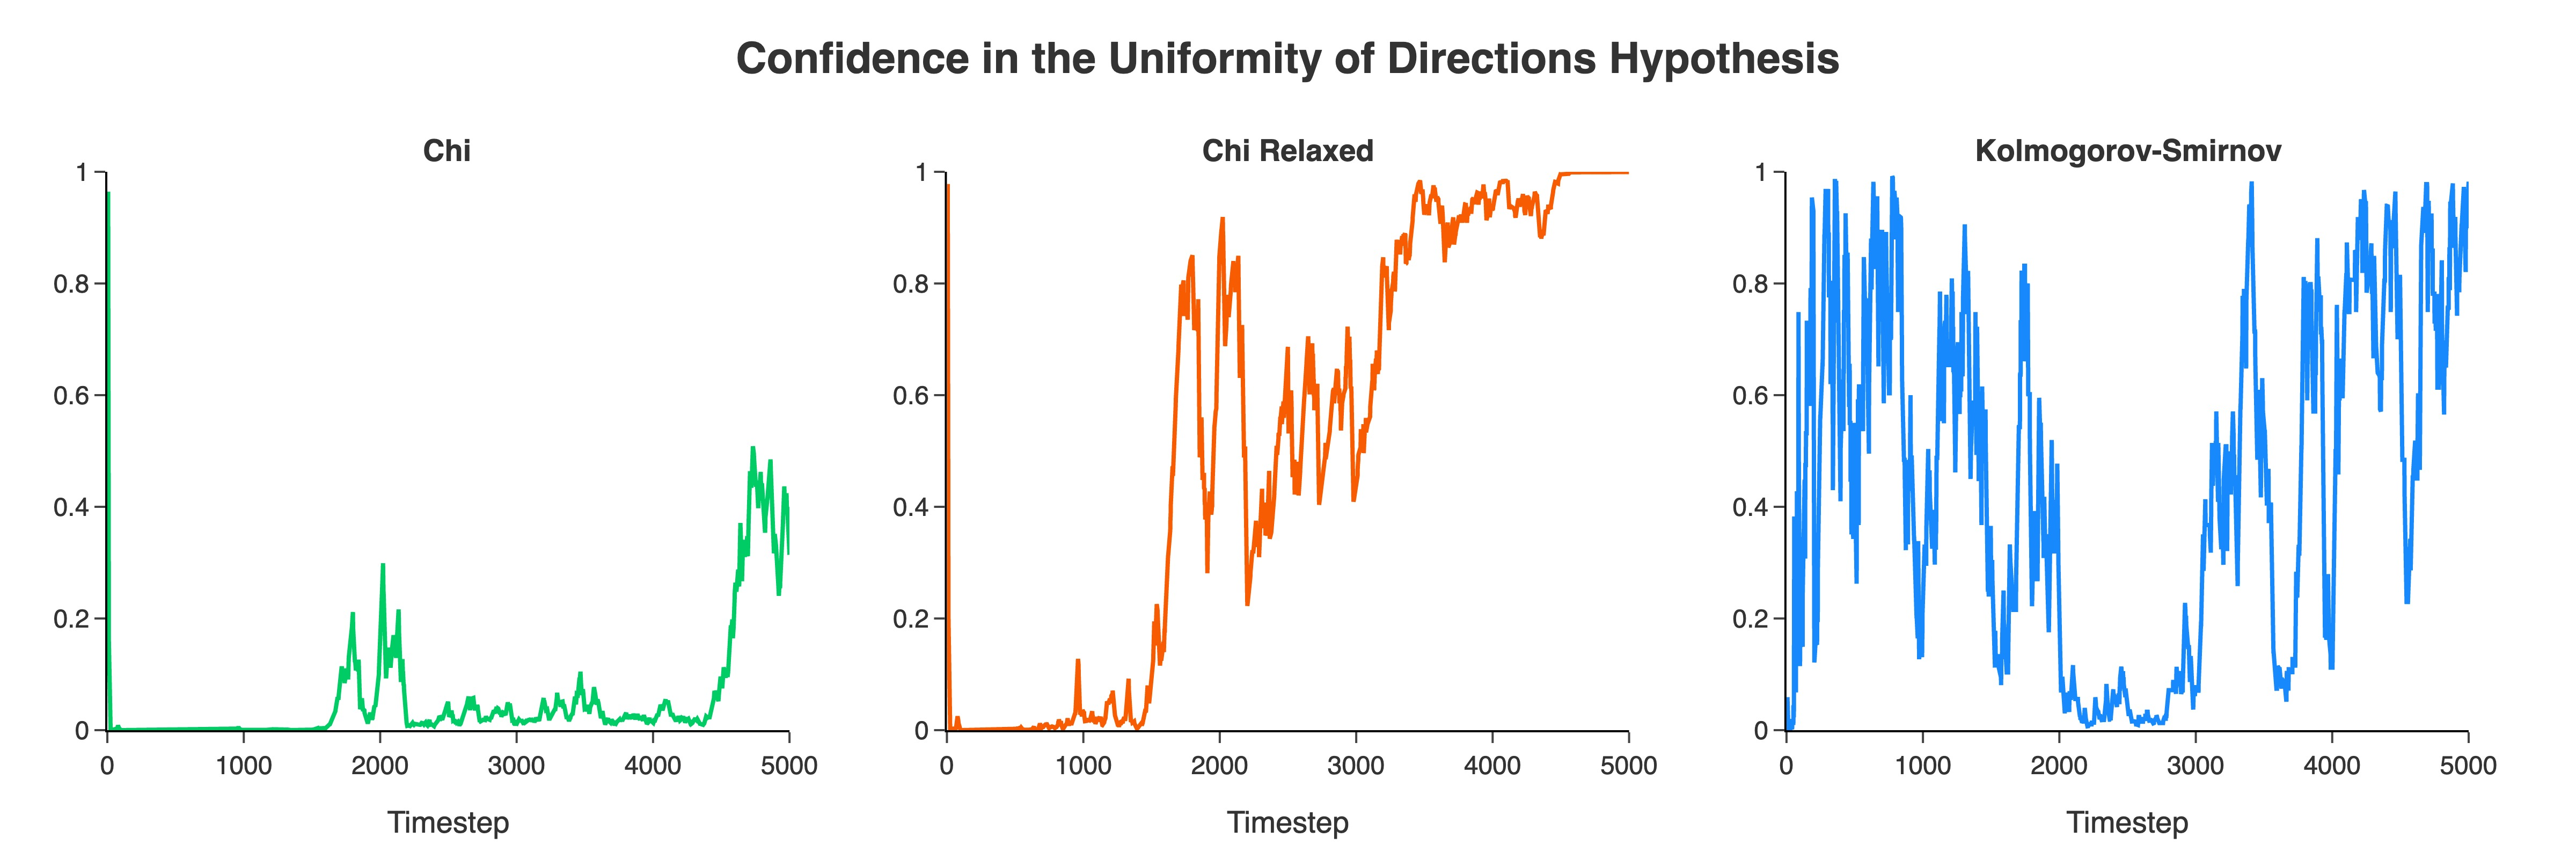
\includegraphics[width=\linewidth]{../figures/jpg/uniformity/atoms_1000_temp_10000_uniformity_confidence.jpg}
    % \end{minipage}
    \caption{Thermal equilibration of carbon and oxygen atoms separated by a rigid wall that only permits energy exchange. The initial temperature for carbon atoms is set to $T=\qty{300}{K}$, and the initial temperature for oxygen atoms is set to $T=\qty{4000}{K}$.}
    \label{fig:rigid_wall}
\end{figure}



\section{Changelog from Midterm Report}
\label{sec:changelog}

The previous iteration of this project had a crucial bug in the collision resolution algorithm. The bug was that the collision resolution algorithm was not treating collisions between particles of different masses correctly, resulting in the explosion of speeds and thus temperatures after sufficient timesteps. The bug was fixed, and the whole codebase was refactored to make it more modular and easier to read. All the results reported were obtained with the new codebase. Finally, let's revisit the future work section from the midterm report and update the statuses of each suggestions.
\begin{itemize}
    \itemsep-0.1em
    \item \textbf{\textcolor{green}{DONE}}: Find the mistake in the simulation algorithm
    \item \textbf{\textcolor{green}{DONE}}: Expand the UI of the simulation to allow for more customization: choosing elements, initial temperatures, numbers of atoms. 
    \item \textbf{\textcolor{orange}{PARTIALLY}}: Perform the simulation (once implemented correctly) with different number of particles and see whether the magnitude of fluctuations in temperature scales as $1/\sqrt{N}$. \textit{the temperature fluctuations seem to be constant at around 10\% regardless of the number of particles. Perhaps this could be attributed to the insufficient time of the simulation and the system not reaching equilibrium in 5000 steps. It should be noted that with 10 000 atoms even 5000 steps take 2 hours of wall time for a single temperature.}
    \item \textbf{\textcolor{orange}{PARTIALLY}}: Perform the simulation with different initial temperatures and see whether the final temperature matches the one predicted by the heat transfer equation. \textit{the final temperature seems to be close to the average of the initial temperatures of the two sets of particles when the number of particles is the same and masses of particles are comparable. A more rigorous assessment should be performed.}
    \item \textbf{\textcolor{blue}{FUTURE WORK}}: Investigate inelastic collisions.
    \item \textbf{\textcolor{blue}{FUTURE WORK}}: Introduce the potential energy term into the simulation. That is, add interatomic interactions.
    \item \textbf{\textcolor{green}{DONE}}: Trace a trajectory of movement of a single particle in the box.
    \item \textbf{\textcolor{green}{DONE}}: Make particles to have non-zero volume. I.e. have particles with different sizes.
    \item \textbf{\textcolor{blue}{FUTURE WORK}}: Explore whether we can model chemical reactions.
    \item \textbf{\textcolor{orange}{PARTIALLY}}: Introduce unit tests for significant parts of the code.
    \item \textbf{\textcolor{orange}{PARTIALLY}}: Improve documentation.
\end{itemize}

\section{Detailed Methodology}
\label{sec:methods-detailed}
I define a class \texttt{Particle} which stores particle position $(x,y)$ and velocities $v_x,v_y$. Coordinates $(x,y)$ are drawn independently from a uniform distribution defined by the compartments of the box. Velocities are initialized as $v_x=v_0 \cos \phi$ and $v_y=v_0 \sin \phi$ where $\phi=2\pi n$ where $n$ is drawn from a uniform distribution $[0,1]$. The $v_0$ is set to be the most probable speed (as determined by the Maxwell-Boltzmann distribution) given the particle mass and initial temperature. An important method of the Particle class is \texttt{move} which updates the position of the particle according to its velocity:
\begin{align}
    x_t &= x_{t-1} + v_x & y_t &= y_{t-1} + v_y
\end{align}
Right now, \texttt{move} method also reflects the velocity components if the particle hits the wall.

The \texttt{check\_collision} method in the Particle class determines and handles collisions between particles $(m_1, r_1, \vec{q}_1, \vec{v}_1)$ and $(m_2, r_2, \vec{q}_2, \vec{v}_2)$ where $m_i$, $r_i$, $\vec{q}=(q_x, q_y)$, $\vec{v}=(v_x,v_y)$ are the mass, radius, position and velocity of the particle. A Euclidean distance between two particles is computed as $d=\sqrt{(q_{1x}-q_{2x})^2+(q_{1y}-q_{2y})^2}$. If the distance is less than the sum of the radii $r_1+r_2$, the particles are considered to be colliding. The collision is resolved by updating the velocities of the particles according to the following equations:
\begin{align}
\vec{v}_1^{\;(t)} &= \vec{v}_1^{\;(t-1)} - \frac{2  m_2}{m_1+m_2} \cdot \frac{\langle \vec{v}_1^{\;(t-1)} - \vec{v}_2^{\;(t-1)}, \vec{q}_1^{\;(t-1)} - \vec{q}_2^{\;(t-1)} \rangle}{\| \vec{q}_1^{\;(t-1)} - \vec{q}_2^{\;(t-1)} \|^2} \cdot (\vec{q}_1^{\;(t-1)} - \vec{q}_2^{\;(t-1)}) \\
\vec{v}_2^{\;(t)} &= \vec{v}_2^{\; (t-1)} - \frac{2  m_1}{m_1+m_2} \cdot \frac{\langle \vec{v}_2^{\;(t-1)} - \vec{v}_1^{\;(t-1)}, \vec{q}_2^{\;(t-1)} - \vec{q}_1^{\;(t-1)} \rangle}{\| \vec{q}_1^{\;(t-1)} - \vec{q}_2^{\;(t-1)} \|^2} \cdot (\vec{q}_2^{\;(t-1)} - \vec{q}_1^{\;(t-1)})
\end{align}

\subsection*{\texttt{TwoCompartments}}
This class models a system with two compartments containing particles. It provides functionality for initializing the system and simulating its behavior:

\begin{itemize}
    \itemsep-0.2em
    \item \texttt{\_\_init\_\_}: Initializes the system with configurable parameters such as the number of particles, atom types, temperatures, and physical properties of each compartment.
    \item \texttt{particles}: A property that returns a \texttt{ParticleIterable} instance to iterate over all particles in both compartments.
    \item \texttt{reset}: Resets the system to its initial state based on the parameters provided during initialization.
    \item \texttt{update}: Advances the system by one time step, updating the state of all particles and performing necessary calculations like collision detection and statistical analyses.
    \item \texttt{update\_compartment\_fractions}: Calculates the fraction of a specific type of particle in each compartment.
    \item \texttt{compute\_velocity\_distribution}: Analyzes the velocity distribution of particles in each compartment.
    \item \texttt{assess\_uniformity}: Evaluates the uniformity of particle distribution and motion.
    \item \texttt{find\_equipartition\_temperature}: Determines the temperature distribution among particles based on their kinetic energy.
    \item \texttt{export\_statistics} and \texttt{export\_particles}: these methods are called by the server to update the GUI.
    \item \texttt{analyze\_game}: Generates and saves visual representations of various statistical analyses of the system.
\end{itemize}

A more detailed description of the most important methods follows:
\subsection*{\texttt{update}}
This method advances the system simulation by one time unit. It involves the following steps:
\begin{itemize}
    \itemsep-0.2em
    \item Increment the internal time counter.
    \item Reinitialize the Quadtree structure if the \texttt{use\_quadtree} flag is True.
    \item Move each particle and check for wall collisions if a rigid wall is present.
    \item Insert particles into the Quadtree.
    \item Perform collision checks between particles. This is done either using the Quadtree (if \texttt{use\_quadtree} is True) or by directly comparing all pairs of particles.
    \item Periodically (based on \texttt{update\_frequency}), update compartment fractions, recalculate equipartition temperature, compute velocity distributions, assess uniformity, and adjust the most probable speed frequency.
\end{itemize}

\subsection*{\texttt{compute\_velocity\_distribution}}
This method analyzes the velocity distribution of particles. It operates differently depending on whether it's the initial computation or a subsequent one:
\begin{enumerate}
    \itemsep-0.2em
    \item If initial, it sets up the velocity bins and assigns all particles to the middle bin.
    \item If not initial, it calculates the velocity distribution of particles, placing them into appropriate bins based on their speeds. The distribution is normalized to reflect relative frequencies.
    \item The velocity distribution is computed separately for each compartment and stored for further analysis.
\end{enumerate}

\subsection*{\texttt{assess\_uniformity}}
This method evaluates the uniformity of particle movement angles (directions). Key steps include:
\begin{enumerate}
    \itemsep-0.2em
    \item Calculating the angle of velocity for each particle.
    \item Binning these angles to assess their distribution.
    \item Performing statistical tests (Chi-square and Kolmogorov-Smirnov) to determine if the distribution of angles follows a uniform distribution, indicating random motion. The relaxed chi-square statistic computes the chi-square statistic as:
    \begin{align}
        \chi^2 = \sum_i \frac{ (\text{max} \left( \vert O_i - E_i\vert - 0.05\times E_i, 0  \right))^2}{E_i}
    \end{align}
    \item Storing the p-values from these tests for analysis.
\end{enumerate}

\subsection*{\texttt{find\_equipartition\_temperature}}
This method calculates the equipartition temperature of particles in each compartment based on their kinetic energies. Steps include:
\begin{enumerate}
    \itemsep-0.2em
    \item Calculating the total kinetic energy of particles in each compartment.
    \item Using the equipartition theorem to determine the temperature corresponding to this energy. Specifically,
    \begin{align}
        \langle KE \rangle = \frac{3}{2} k_B T = \frac{1}{2} m \sum_i v_i^2 \implies T = \frac{m}{3k_B N} \sum_i v_i^2
    \end{align}
    \item Storing the temperature values for further analysis and comparison.
\end{enumerate}


\subsection*{Description of the \texttt{EnergyWall} Class}
This class models a physical barrier between compartments that can absorb, store, and emit energy when particles collide with it. It provides functionality for interacting with particles and updating its internal state.

\subsubsection*{Attributes}
\begin{itemize}
    \itemsep-0.2em
    \item \texttt{position} (float): The position of the wall.
    \item \texttt{stored\_energy} (float): The energy currently stored in the wall.
    \item \texttt{energy\_limit} (float): The maximum energy capacity of the wall.
    % \item \texttt{interaction\_count} (int): Count of interactions with particles.
    \item \texttt{moving\_alpha} (float): Factor for calculating the running average of energy.
    \item \texttt{running\_average} (float): The running average of the energy absorbed from particles.
\end{itemize}


\subsubsection*{Method: \texttt{interact\_with\_particle(self, particle)}}
Handles interactions between the wall and a particle. The process is as follows:
\begin{enumerate}
    \itemsep-0.2em
    \item Calculate the kinetic energy of the interacting particle.
    \item Determine if the wall should absorb or emit energy based on the particle's energy and the wall's stored energy. Emit energy if the particle's kinetic energy is less than the wall's running average energy, and the wall's stored energy is at least 80\% of its energy limit. Absorb energy if the particle's kinetic energy is greater than the average or if the wall's stored energy is below its energy limit.
    \item \textbf{Energy Emission:} The energy transfer is a fraction (10\% in the implementation) of the difference between the wall's average energy and the particle's kinetic energy, capped at the wall's current stored energy.
    \item \textbf{Energy Absorption:} The wall updates its running average using the \texttt{moving\_alpha} factor. The energy absorbed is the lesser of 10\% of the excess kinetic energy of the particle or the remaining capacity of the wall.
    \item Adjust the particle's velocity to reflect the change in kinetic energy, or simply reverse its horizontal velocity if no energy transfer is needed.
\end{enumerate}




\end{document}